\documentclass{article}

\def\shownotes{1}

\usepackage{natbib}
\setcitestyle{authoryear,open={(},close={)}}
\renewcommand{\cite}{\citep}
\newcommand{\yell}[1]{{\color{red}#1}}
\newcommand*\samethanks[1][\value{footnote}]{\footnotemark[#1]}
\usepackage{authblk}
\usepackage[margin=1in]{geometry}
%\usepackage{hyperref}

\usepackage{macro_math}
\usepackage[us,12hr]{datetime} % `us' makes \today behave as usual in TeX/LaTeX
\usepackage{graphicx, subcaption}
\usepackage[export]{adjustbox}
\usepackage{subfloat}
\usepackage[T1]{fontenc}    %
\usepackage{nicefrac}       %
\usepackage{microtype}      %
\usepackage[hidelinks]{hyperref}
\hypersetup{colorlinks,linkcolor={blue},citecolor={blue},urlcolor={red}}
\usepackage{macro_fan}
\usepackage{stmaryrd}
\usepackage[utf8]{inputenc} %
\usepackage{caption,subcaption}

%\newcommand{\citet}{\cite}

\begin{document}

	\title{Analyzing Information Transfer from Different Data Sources via Precise Bias-variance Asymptotics}
	\iffalse
	\vspace{0.15in}
	\author[1]{Hongyang R. Zhang\thanks{HZ and FY contributed equally to the theoretical results. SW conducted the experimental analysis. Correspondence to hrzhang@northeastern.edu or fyang75@wharton.upenn.edu.}}
	\author[2]{Fan Yang\samethanks}
	\author[3]{Sen Wu\samethanks}
	\author[2]{Weijie J. Su}
	\author[3]{Christopher R\'e}
	\vspace{0.15in}
	\affil[1]{Khoury College of Computer Sciences, Northeastern University}
	\affil[2]{Department of Statistics, The Wharton School, University of Pennsylvania}
	\affil[3]{Department of Computer Science, Stanford University}
	\fi

	\maketitle
	\begin{abstract}
%	Hard parameter sharing for multi-task learning is widely used in empirical research despite the fact that its generalization properties have not been well established in many cases. This paper studies its generalization properties in a fundamental setting: How does hard parameter sharing work given multiple linear regression tasks? We develop new techniques and establish a number of new results in the high-dimensional setting, where the sample size and feature dimension increase at a fixed ratio. First, we show a sharp bias-variance decomposition of hard parameter sharing, given multiple tasks with the same features. Second, we characterize the asymptotic bias-variance limit for two tasks, even when they have arbitrarily different sample size ratios and covariate shifts. We also demonstrate that these limiting estimates for the empirical loss are incredibly accurate in moderate dimensions. Finally, we explain an intriguing phenomenon where increasing one task's sample size helps another task initially by reducing variance but hurts eventually due to increasing bias. This suggests progressively adding data for optimizing hard parameter sharing, and we validate its efficiency in text classification tasks.
\end{abstract}

	% The idea is to use a shared feature space for all tasks, while each task also has a separate layer for making the prediction.
\begin{abstract}
	Hard parameter sharing for multi-task learning is widely used in empirical research despite the fact that their generalization properties have not been established in many cases. This paper studies a fundamental question to better understand this approach: How does hard parameter sharing work given multiple linear regression tasks? We develop new techniques and establish a number of new results in the high-dimensional setting, where the sample size and feature dimension become increasingly large in a fixed ratio. First, we show a sharp bias-variance decomposition of hard parameter sharing, given multiple tasks with the same features. Second, we characterize the asymptotic bias-variance limit for two tasks, even when they have arbitrarily different sample size ratios and covariate shifts. We also demonstrate that these limiting estimates for the empirical loss are incredibly accurate in moderate dimensions. Finally, we explain an intriguing phenomenon where increasing one task's sample size helps another task initially by reducing variance but hurts eventually due to increasing bias. This suggests progressively adding data for optimizing hard parameter sharing, and we validate its efficiency in text classification tasks.
\end{abstract}

\section{Introduction}\label{sec introduction}

\iffalse
%Multi-task learning is an inductive learning mechanism to improve generalization performance using related task data.
%Many state-of-the-art results in computer vision and natural language processing are obtained using multi-task learning.
Multi-task learning is a powerful approach to improve performance for many tasks in computer vision, natural language processing, and other areas \cite{C97,ZY17,R17}.
%In multi-task learning, having related task data is fundamental to its performance.
%Multi-task learning is particularly powerful when there is limited labeled data for a task to be solved, meanwhile more labeled data from different but related tasks is available.
%By combining multiple information sources, it is possible to share all the information in the same model.
In many settings, multiple source tasks are available to help with predicting a particular target task.
\todo{clarify setting is different from traditional MTL}
%For example, many applications in , and many other areas have been achieved by learning from multiple tasks together.
The performance of multi-task learning depends on the relationship between the source and target tasks \cite{C97}.
%	We define that multi-task learning provides \textit{positive transfer} if it outperforms single-task learning, or \textit{negative transfer} otherwise.
When the sources are relatively different from the target, multi-task learning (MTL) has often been observed to perform worse than single-task learning (STL) \cite{AP16,BS17}, which is referred to as \textit{negative transfer} \cite{PY09}.
While many empirical approaches have been proposed to mitigate negative transfer \cite{ZY17}, a precise understanding of when negative transfer occurs remains elusive in the literature \cite{R17}.
%This phenomenon, known as \textit{negative transfer}, is fundamental to the understanding of multi-task learning.

%Inspired by the theory, we propose an incremental training schedule to improve multi-task training.
%We consider a setting where the target task has limited labeled data and show
%On the other hand, unless the structures across task data are well-understood, applying multi-task learning on several different datasets often result in suboptimal models (or negative transfer in more technical terms).

Understanding negative transfer requires developing generalization bounds that scale tightly with properties of each task data, such as its sample size.
This presents a technical challenge in the multi-task setting because of the difference among task features, even for two tasks.
ithout a tight lower bound for multi-task learning, comparing its performance to single-task learning results in vacuous bounds.
\todo{add more technical motivation (or maybe later)}
From a practical standpoint, developing a better understanding of multi-task learning in terms of properties of task data can provide guidance for downstream applications \cite{RH19}.
%For example,
%On the other hand, uneven sample sizes (or dominating tasks) have been empirically observed to cause negative transfer \cite{YKGLHF20}.
%The benefit of learning multi-task representations has also been studied for certain half-spaces \cite{} and sparse regression \cite{}.
%When all tasks are sufficiently similar, adding more labeled data improves the generalization performance for predicting a particular task \cite{WZR20}.

%\textbf{Setup and Main Results.}
In this work, we study the bias and variance of multi-task learning in the high-dimensional linear regression setting \cite{HMRT19,BLLT20}.
Our key observation is that three properties of task data, including \textit{task similarity}, \textit{sample ratio}, and \textit{covariate shift}, can affect whether multi-task learning outperforms single-task learning (which we refer to as \textit{positive transfer}).
As an example, we vary each property in Figure \ref{fig_model_shift_phasetrans} for two linear regression tasks and measure the improvement of multi-task learning over single-task learning for a particular task.
We observe that the effect of transfer can be either positive or negative as we vary each property.
These phenomena cannot be explained using previous techniques \cite{WZR20}.
The high-dimensional linear regression setting allows us to measure the three properties precisely.
Here we define each property for the case of two tasks, while our definition applies to general settings.
We refer to the first task as the source task and the second as the target task.
\squishlist
	\item \textbf{Task similarity:} Assume that both tasks follow a linear model with parameters $\beta_1, \beta_2\in\real^p$, respectively.
	We measure the distance between them by $\norm{\beta_1 - \beta_2}$.
	\item \textbf{Sample ratio:} Let $n_1 = \rho_1 \cdot p, n_2 = \rho_2 \cdot p$ be the sample size of each task, where $\rho_1, \rho_2>1$ are both fixed values that do not grow with $p$.
	We measure the source/target sample ratio by $\rho_1 / \rho_2$.
%	Importantly, $\rho_2$ can be a small constant (say $2$) to capture the need for more labeled data.
	\item \textbf{Covariate shift:} Assume that the task features are random vectors with positive semidefinite covariance matrices $\Sigma_1\in\real^{p\times p}$ and $\Sigma_2\in\real^{p\times p}$, respectively.
	%$x = \Sigma_i^{1/2}z$, where $z\in\real^p$ consists of i.i.d. entries with mean zero and unit variance, and is a positive semidefinite matrix.
	We measure covariate shift with matrix $\Sigma_1^{1/2}\Sigma_2^{-1/2}$.
\squishend
\fi


Hard parameter sharing (HPS) for multi-task learning is widely used in empirical research and goes back to the seminal work of \citet{C97}.
Recent work has revived interest in this approach because it improves performance and reduces the cost of collecting labeled data \cite{MTDNN19,ZSSGM18}.
It is generally applied by sharing the feature layers between all tasks while keeping an output layer for every task.
Often, hard parameter sharing offers two critical advantages if successfully applied.
(i) It reduces model parameters since all tasks use the same feature space.
(ii) It reduces the amount of labeled data needed from each task by augmenting the entire training dataset.

Hard parameter sharing offers great intuitive appeal as an inductive transfer mechanism.
It reduces overfitting by acting as a regularizer \cite{R17}.
For example, by restricting the shared space's size, HPS encourages information sharing among multiple tasks \cite{KD12}.
Another source of inductive bias comes from the tasks and depends on datasets' properties such as sample sizes and task covariances \cite{WZR20}.
However, how these dataset properties impacts HPS has not been established.
%It becomes increasingly important to understand HPS' formal generalization properties.
Part of the challenge may be that HPS' generalization performance depends intricately on the sample size ratios and covariate shifts between tasks, not amenable to standard concentration results.
Previous results based on Rademacher complexity or VC dimensions have considered when all tasks' sample sizes are equal to logarithm factors of feature dimension \cite{B00,MPR16}, and when all tasks' sample sizes increase simultaneously \cite{AZ05,M06}.
%For, the generalization error scales down as the sample sizes of all tasks increase, when applied to the multi-task setting \cite{B00,AZ05,M06,MPR16,WZR20}.

This paper presents new techniques to study hard parameter sharing and establish a number of new results.
We consider regression analysis, which is arguably one of the most fundamental problems in statistics and machine learning.
We are interested in the \textit{high-dimensional} setting, where each dataset's sample size and feature dimension grow linearly at a fixed ratio.
This is motivated by many multi-task learning applications, where the amount of labeled data from each dataset is usually insufficient for learning a single task.
For example, this is the case if a dataset's sample size is only a small constant factor of the feature dimension.
The high-dimensional setting is challenging but is crucial for understanding how datasets' sample sizes impact generalization performance.

	\subsection{Problem Formulation and Main Results}

%Suppose we have $t$ labeled regression tasks. %where $t$ is a fixed value that does not grow with the feature dimension $p$.
%For each task $k$ from $1$ to $t$, we have $n_k$ samples $x_1, x_2, \dots, x_{n_k}$ that are all $p$-dimensional feature vectors with real-valued labels $y_1, y_2, \dots, y_{n_k}$.
%Without loss of generality, we focus on predicting the $t$-th task and refer the $t$-th task as the target.
%We refer to task $1$ to task $t-1$ as source tasks.
%We assume that the labels of each task $k$ satisfy the linear model with unknown parameters $\beta_k\in\real^p$, that is,
%	\[ y_i = x_i^{\top}\beta_k + e_i, \text{ for all } 1 \le i \le n_k, \]
%where $e_i$ denotes random noise with mean zero and variance $\sigma^2$.
%To write the above notations more succiently, let $X_k \in \real^{n_k \times p}$ denote the covariates that consists of a feature vector in every row.
%Let
%	\be\label{model_YvsX} Y^{(k)} = X^{(k)} \beta_k + \varepsilon_k, \text{ for all } 1\le k \le t \ee denote the label vector of task $k$ and $\varepsilon_k$ denote an i.i.d. random vector with mean zero and variance $\sigma^2$.
%Following \citet{HMRT19} and \citet{BLLT20},
%In the high-dimensional linear regression setting (e.g. ), the features of the $k$-th task, denoted by $X_k\in\real^{n_i\times p}$, consist of $n_k$ feature vectors given by $x_1, x_2, \dots, x_{n_k}$.
%we assume that for each task $k$ from $1$ to $t$, each feature vector $x_i = \Sigma^{1/2}_k z_i$ for $i = 1, \dots, n_k$, where $z_i\in\real^p$ is an i.i.d. random vector with  mean zero and unit variance.
%Recall that $\Sigma_k$ is the population covariance matrix task $k$'s feature vectors.
%Let $\Sigma_k = U_k D_k U_k^{\top}$ denote the singular value decomposition of $\Sigma_k$.
%We denote $\Sigma_k = U_k D_k^{1/2}$ as the square root of $\Sigma_k$.
%The sample size of task $k$, given by $n_k$, is equal to $\rho_k\cdot p$ for a fixed value $\rho_k$ that does not grow with feature dimension $p$.
%This setting is also known as the high-dimensional linear regression setting in the literature.
%There are two motivations for studying the high-dimensional linear regression setting for multi-task learning.
%First, this setting captures salient properties of modern large-scale datasets, where the sample sizes are usually on the order of tens to hundreds of the number of features \cite{sur2019modern}.
%Second, as we will see soon in Section \ref{sec_general}, we can derive precise asymptotics of the generalization error that scale with properties of the task data such as sample sizes.
%The labels $Y_k = X_k \beta_k + \varepsilon_k$, where $\beta_k$ denotes the linear model parameters and $\varepsilon_k$ denotes i.i.d. noise with mean zero and variance $\sigma^2$.
%Recall that we have $t$ labeled training datasets, denoted by $(X_1, Y_1), (X_2, Y_2), \dots, (X_t, Y_t)$, where $X_i\in\real^{n_i\times p}$ and $Y_i\in\real^{n_i}$ for $1\le i\le t$.
%Following \cite{HMRT19,BLLT20}, we assume that for each task $i = 1,2,\dots,t$,  every feature vector is generated as $x = \Sigma_i^{1/2} z$, where $z\in\real^p$ is a random vector with i.i.d. entries of mean zero and unit variance and $\Sigma_i\in\real^{p\times p}$ is a positive semidefinite matrix.
%Without loss of generality, let the $t$-th task be the target task.

Regression analysis is arguably one of the most fundamental methods in statistics and machine learning.
In many multi-task learning applications, the amount of labeled data from each dataset is usually insufficient for learning a single task.
For example, this is the case if a dataset's sample size is only a small constant factor of the feature dimension \cite{GLUE}.
In this paper, we consider multi-task learning in a \textit{high-dimensional} linear regression setting, where each dataset's sample size and the feature dimension grow linearly at a fixed ratio.
The high-dimensional setting is challenging but is crucial for understanding how datasets' sample sizes impact generalization performance.
We assume that there are multiple datasets that all follow a (potentially different) linear model.
In each dataset, suppose the feature vector $x = {\Sigma}^{1/2} z$, where $z \in \real^p$ has i.i.d entries with mean zero, unit variance, and covariance $\Sigma \in\real^{p \times p}$ that is deterministic and positive semidefinite.

We study a hard parameter sharing architecture to learn jointly from multiple datasets.
In this architecture, there is a shared feature representation layer $B\in\real^{p\times r}$ for all tasks and a separate output layer $A_i \in \real^r$ for every task $i$.
Suppose we have $t$ datasets.
For each dataset $i$ from $1$ to $t$, let $n_i$ denote its sample size, $X^{(i)} \in \real^{n_i \times p}$ denote its feature covariates, and $Y^{(i)} \in \real^{n_i}$ denote all the labels.
%The width of $B$, denoted by $r$, plays an important role in regularization.
%As observed in Proposition 1 of \citet{WZR20}, if $r \ge t$, there is no regularization effect.
%Hence, we assume that $r < t$ in our study.
%For example, when there are only two tasks, $r = 1$ and $B$ reduces to a vector whereas $W_1, W_2$ become scalars.
Let $A = [A_1, A_2, \dots, A_t] \in \real^{r \times t}$.
We study the following optimization objective.
%	\item Separate each dataset $(X_i, Y_i)$ randomly into a training set $(X_i^{tr}, Y_i^{tr})$ and a validation set $(X_i^{val}, Y_i^{val})$.
%	The size of each set is described below.
%	\item Learn the shared layer $B$: minimize the training loss over $B$ and $W_1, \dots, W_t$, leading to a local minimum of $B$ that depends on $W_1, \dots, W_t$, denoted by $\hat{B} = \hat{B}(W_1, \dots, W_t)$.
\begin{align}\label{eq_mtl}
			f(A, B) = \sum_{i=1}^t \norm{X^{(i)} B A_i - Y^{(i)}}^2.
\end{align}
Given a solution $\hat{A}, \hat{B}$ from the above optimization, let $\hat{\beta}_i^{\MTL} = \hat{B} \hat{A}_i$ denote the hard parameter sharing (HPS) estimator for task $i$.
The critical questions here are:
(i) how well does the estimator work? In particular, how does the performance of the estimator scale with sample size?
(ii) for datasets with different sample sizes and covariate shifts, how do they impact the estimator?


%	\item Learn the output layers $W_1, W_2, \dots, W_t$: set $B = \hat{B}$ and minimize the training loss over $W_1, W_2, \dots, W_t$.
%		{\begin{align}\label{eq_mtl_eval}
%			g(W_1, \dots, W_t) = \sum_{k=1}^t \norm{X_k \hat{B} W_k - Y_k}^2.
%		\end{align}}
%\end{enumerate}
%Let $\hat{\beta}_t^{\MTL}$ denote the multi-task learning estimator obtained from the procedure above.
%By contrast, let $\hat{\beta}_t^{\STL} = (X_t^{\top}X_t)^{-1}X_t^{\top}{Y_t}$ denote the single-task learning estimator. % denoted by $L(\hat{\beta}_t^{\STL})$.
%where $B\in\real^{p\times r}$ and $W_k\in\real^r$ for every $1\le k\le t$.
%Following , we assume that $r < t$, because otherwise minimizing $f(\cdot)$ could result in $BW_i$ being the single-task optimum.
%\smallskip
%\noindent\textit{Remark.}
%In general, the multi-task learning objective $f(\cdot)$ is non-convex with respect to $B$ and $W_1, \dots, W_t$.
%Therefore, we first minimize $B$ in equation \eqref{eq_mtl} and then minimize $W_k$ given $B$ in equation \eqref{eq_mtl_eval}.
%For our results later in Section \ref{sec_general} and \ref{sec_special}, we will identify tractable cases and provide guarantees to the above procedure.
%\paragraph{Problem statement.}
%We focus on predicting a particular task, say the $t$-th task, without loss of generality.
%For an estimator $\hat{\beta}$ of the target task model $\beta_t$, we define the prediction loss of the estimator $\hat{\beta}$ as
%	{\begin{align}\label{eq1_prediction_loss}
%		\te(\hat{\beta}) = \exarg{x = \Sigma_t^{1/2} z}{({x}^{\top}\hat{\beta} - {x}^{\top}\beta_t)^2}
%		= \bignorm{\Sigma_t^{1/2} (\hat{\beta} - \beta_t)}^2,
%	\end{align}}%
%where $x = \Sigma_t^{1/2} z$ denotes a random feature vector with covariance $\Sigma_t$.
%In the above equation, $x^{\top}\beta_t$ is the true label of $x$.
%= (\hat{\beta} - \beta_t)^{\top}\Sigma_t(\hat{\beta} - \beta_t)
%We say that the source tasks provide a \textit{positive transfer} to the target task if the prediction loss of the MTL estimator is lower than that of the STL estimator, that is, if
%	\[ L(\hat{\beta}_t^{\MTL}) > L(\hat{\beta}_t^{\STL}). \]
%On the other hand, we say that the source tasks provide a \textit{negative transfer} to the target task if $L(\hat{\beta}_t^{\MTL}) < L(\hat{\beta}_t^{\STL})$.
%Our goal is to study when the source tasks provide a positive transfer to the target task.
%More specifically, we study how varying properties of task data including task similarity, sample ratio, and covariate shift affects information transfer in multi-task learning.

%We begin by defining our problem setup including the multi-task estimator we study.
%Then, we describe the bias-variance tradeoff of the multi-task estimator and connect the bias and variance of the estimator to \textit{task similarity}, \textit{sample size}, and \textit{covariate shift}.
%Finally, we show a tight concentration bound for the bias and variance quantities using random matrix theory.

%\subsection{Problem Formulation}

%In the worst case, the optimization objective \eqref{eq_mtl} is non-convex in $A$ and $B$ (e.g. matrix completion is a special case for suitably designed $X^{(i)}, Y^{(i)}$).
%Therefore, we work in cases where a global and/or local minimum characterization is possible

\paragraph{Main results.}
Our first result (Theorem \ref{thm_many_tasks}) applies to the multi-label prediction setting where all datasets have the same features, and we want to make multiple predictions (e.g. \cite{hsu2009multi}).
We analyze the global minimum of $f(A, B)$, and provide a sharp generalization bound for its (out-of-sample) prediction loss for any task.
This case is tractable even though in general, $f(A, B)$ is non-convex in $A$ and $B$ (e.g. matrix completion is a special case for suitably designed $X^{(i)}, Y^{(i)}$).
We show that the prediction loss of hard parameter sharing admits a clean bias-variance decomposition.
Our results imply that hard parameter sharing helps by reducing variance compared to single-task learning, but hurts by increasing bias.
Our second result (Theorem \ref{thm_main_RMT}) applies to two tasks with arbitrarily different sample sizes and population covariance matrices.
We analyze the local minimum of $f(A, B)$ and provide a sharp generalization bound for both tasks' prediction loss.
Despite its simplicity, we show several rich phenomena by varying sample sizes and covariate shifts in this setting.
See Figure \ref{fig_intro_sample_size} for an illustration.

\begin{figure}[!t]
	\begin{subfigure}[t]{0.5\textwidth}
		\centering
		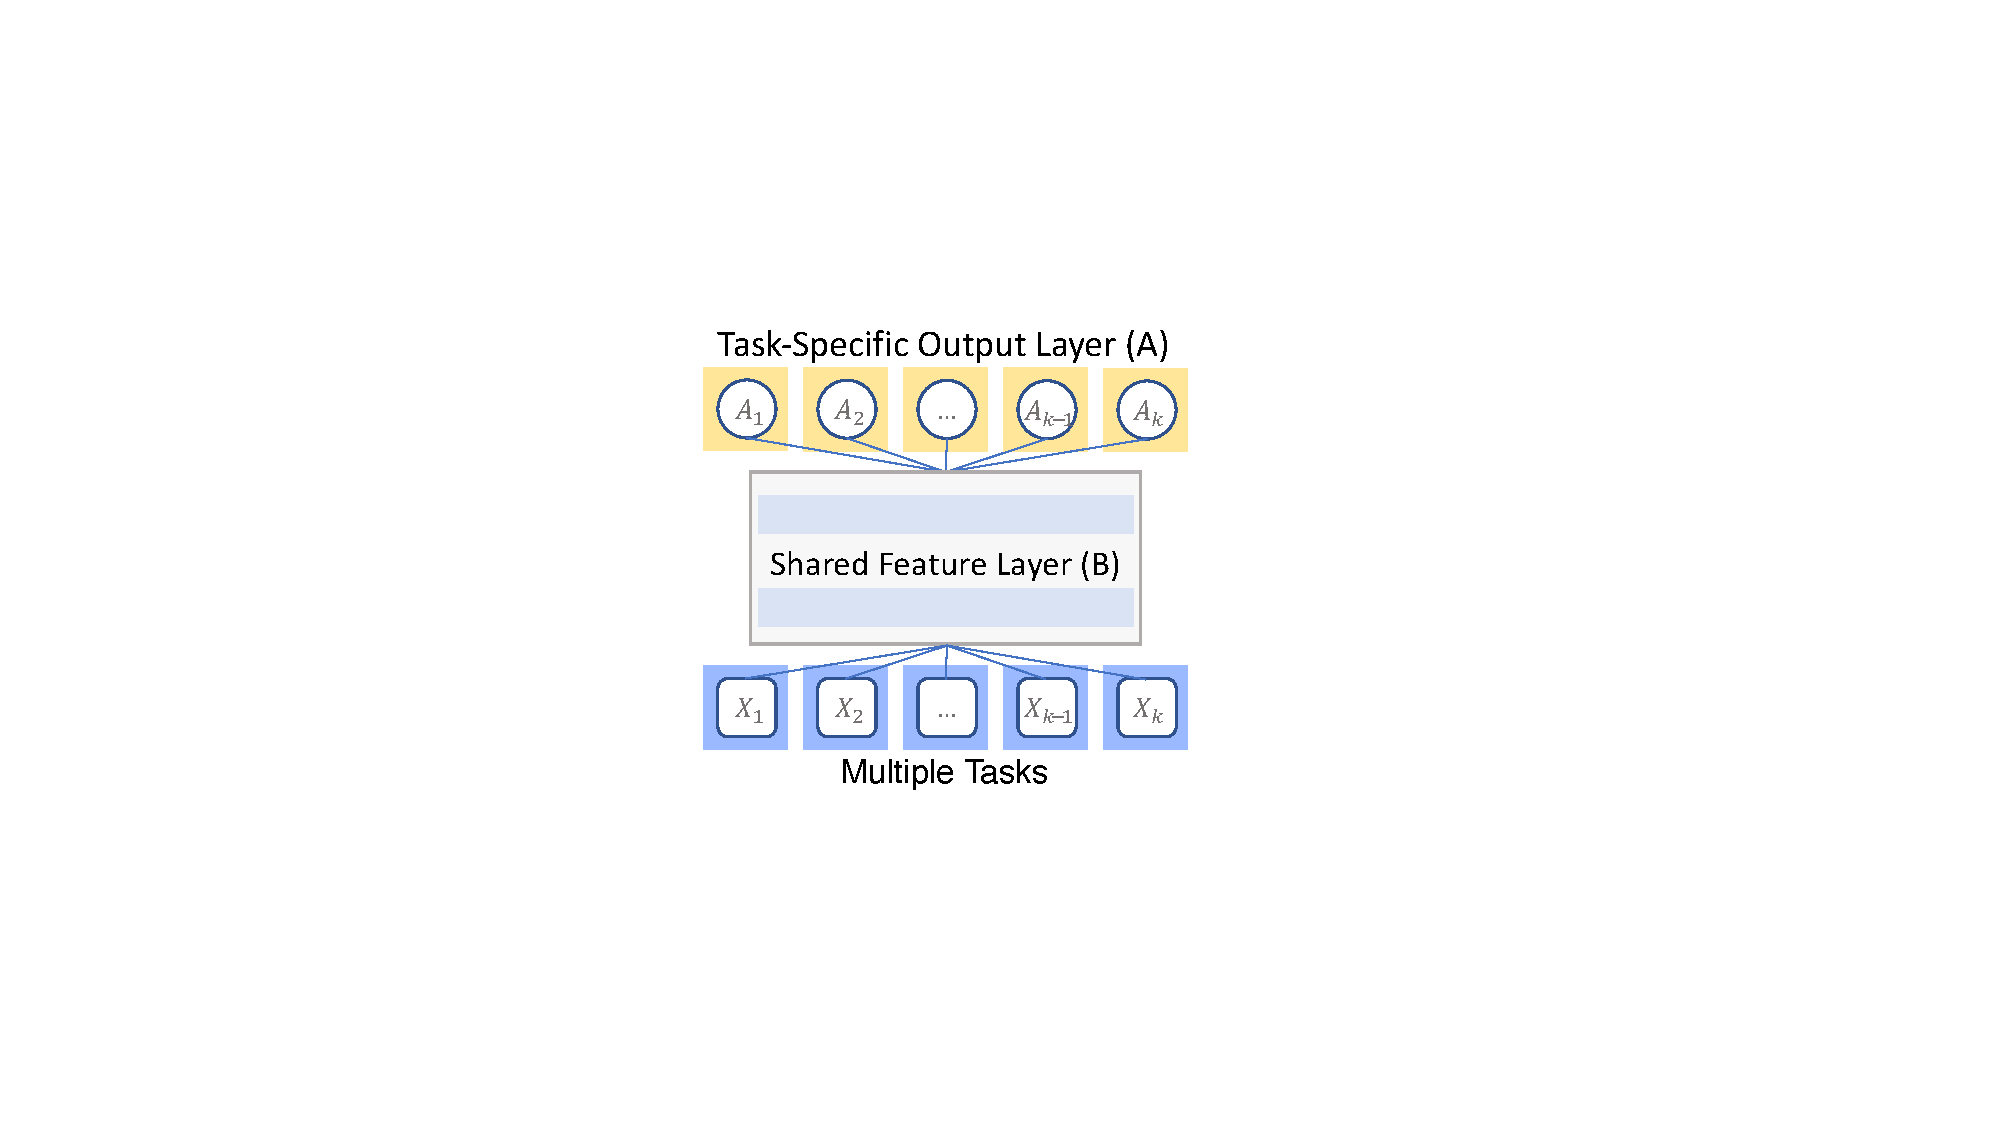
\includegraphics[width=0.5\textwidth,valign=t]{figures/mtl_model_arch.pdf}
		\caption{A hard parameter sharing architecture}
	\end{subfigure}\hfill
	\begin{subfigure}[t]{0.5\textwidth}
		\centering
		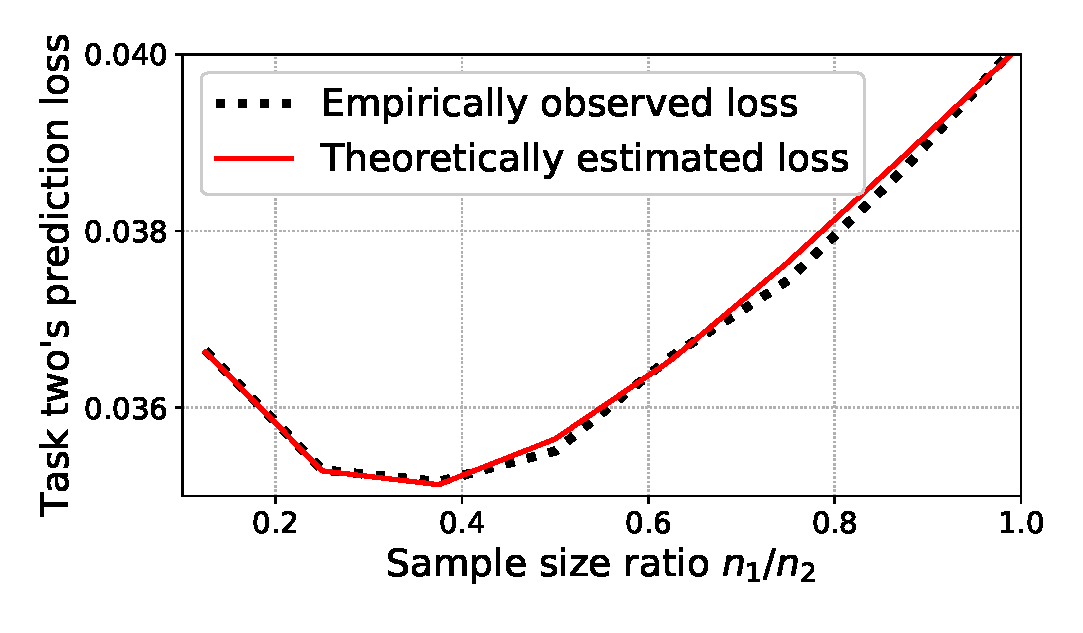
\includegraphics[width=0.713\textwidth,valign=t]{figures/sample_ratio_c2_400.eps}
		\caption{Varying sample size ratio}
		\label{fig_intro_sample_size_b}
	\end{subfigure}
	\caption{An illustrative example of our result:
	Consider the prediction loss of hard parameter sharing (left) for task two, given two linear regression tasks.
	Increasing task one's sample size decreases task two's prediction loss initially, but increases afterward. This phenomenon occurs due to different bias-variance tradeoffs as the sample size ratio increases. Our result provides an estimated loss (solid line) that accurately matches the empirical loss (dotted line).
	See Section \ref{sec_simulation} for the precise setting.}
	\label{fig_intro_sample_size}
\end{figure}

Consequently, we observe qualitative properties of hard parameter sharing for varying datasets' properties using our precise loss estimates.
\begin{enumerate}
	\item \textit{Sample efficiency (Example \ref{ex_same_cov})}:
	One advantage of combining multiple datasets is that the requirement for labeled data reduces compared to STL, a phenomenon that \citet{ZSSGM18} has observed empirically.
	Our results further imply that HPS's sample efficiency depends on model-specific variance vs. noise variance. It is generally high when the noise variance is large compared to model-specific variance across tasks.
	\item \textit{Sample size ratio (Example \ref{ex_sample_ratio})}: Increasing one task's sample size does not always help reduce another task's loss. In a simplified setting, we find that the task loss either decreases first before increasing afterward or decreases monotonically depending on how much bias increases. These two trends result from different tradeoffs between increasing bias and decreasing variance.
	\item \textit{Covariate shift (Example \ref{ex_covshift})}: In addition to sample sizes, variance also scales with the covariate shift between different datasets. For a high sample size ratio, HPS's  variance is smallest when there is no covariate shift. Counterintuitively, for a low sample size ratio, having covariate shifts reduces variance through a complementary spectrum.
\end{enumerate}

%First, we develop tight bounds for the bias and variance of the multi-task estimator for two tasks by applying recent development in random matrix theory \cite{erdos2017dynamical,isotropic,Anisotropic}.
%We observe that the variance of the multi-task estimator is \textit{always smaller} than single-task learning, because of added source task samples.
%On the other hand, the bias of the multi-task estimator is \textit{always larger} than single-task learning, because of model distances.
%Hence, the tradeoff between bias and variance determines whether the transfer is positive or negative.
%We provide a sharp analysis of the \textit{variance} that scales with sample size and covariate shift.
%We extend the analysis to the bias, which \textit{in addition} scales with {task similarity}.
%Combining both, we analyze the bias-variance tradeoff for two tasks in Theorem \ref{thm_main_informal} and extend the analysis to many tasks with the same features in Theorem \ref{thm_many_tasks}.
%For the setting of two tasks, we show how the variance of the multi-task estimator  scales with sample size and covariate shift in the following result.
%\textit{Our first contribution} is to develop a concentration bound that arises naturally from the bias-variance tradeoff of $\hat{\beta}_t^{\MTL}$ for two tasks.
%Let $\hat{\beta}_t^{\STL}$ denote the single-task estimator.
%Without loss of generality, let the $t$-th task denote the target task.
%Importantly, the target task's data size is a fixed constant times $p$ in the high-dimensional setting.
%Hence adding more labeled data can help improve its test performance.
%$B\in\real^{p\times r}$
%$\set{W_i \in \real^{r}}_{i=1}^t$

%Concretely, we show a tight bound on the trace of $(X_1^{\top}X_1 + X_2^{\top}X_2)^{-1}$, which
%Theorem \ref{lem_cov_shift_informal} allows us to analyze the bias-variance tradeoff of the multi-task estimator for two settings:
%(i) two tasks with arbitrary covariate shift; (ii) many tasks with no covariate shift.

%We shall assume that each task data follows a linear model, i.e. $y_i = X_i \beta_i + \varepsilon_i$, $1\le i\le k$.
%Here $\beta_i\in\real^p$ is the model parameter for the $i$-th task.
%Each row of $X_i\in\real^{n_i\times p}$ is assumed to be drawn i.i.d. from a fixed
%distribution with covariance matrix $\Sigma_i$.

%We extend our result to the transfer learning
%in the setting of high-dimensional linear regression.
%by pooling source task representations into the shared body of the hard parameter sharing architecture, following
%setting of Taskonomy by Zamir et al. \cite{ZSSGM18}.
%We prove that the bias of the transfer learning estimator is given by the projection of $\beta_t$ to the orthogonal subspace spanned by $\set{\beta_i}_{i=1}^{t-1}$.
%These results are described more precisely in Section \ref{sec_main}.

%Second, we explain the phenomena in Figure \ref{fig_model_shift_phasetrans} in isotropic and covariate shifted settings.
%We observe that negative transfer occurs as (a) \textit{task similarity}: tasks become more different; (b) \textit{data size}: source/target data size increases.
%\textbf{Task similarity:}
%\textbf{Data sizes:}
%\textbf{Covariate shift:}
%Furthermore, MTL performance is negatively affected when (c) \textit{covariate shift}: the covariance matrices of the two tasks become more different.
%\squishlist
%	\item We provide conditions to predict the effect of transfer as a parameter of model distance $\norm{\beta_1-\beta_2}$ (Section \ref{sec_similarity}).
%	As model distance increases, the bias becomes larger, resulting in negative transfer.
%	Our result predicts most of the empirical observations in Figure \ref{fig_model_shift} correctly.
%	It is crucial that the concentration result in Theorem \ref{lem_cov_shift_informal} is sufficiently precise so that we can explain the transition phenomena in Figure \ref{fig_model_shift} and \ref{fig_size}.
%	The unexplained observations are caused by an error term from the bias.
%	We discuss these in Section \ref{sec_insight}.
%	\item We provide conditions to predict transfer as a parameter of sample ratio $\rho_1/\rho_2$ (Section \ref{sec_data_size}).
%	Adding source task samples helps initially by reducing variance, but hurts eventually due to bias.
	%namely adding more labeled data from the source task does not always improve performance (Proposition \ref{prop_data_size}).
	%Theorem \ref{lem_cov_shift_informal} allows us to compare MTL performance under different covariate shifts.
%	\item For a special case of $\beta_1=\beta_2$, we show that MTL performs best when the singular values of $\Sigma_1^{1/2}\Sigma_2^{-1/2}$ are all equal  (Section \ref{sec_covshift}).
%	Otherwise, the variance reduces less with covariate shift.
%	Our theoretical bound matches the empirical curve in Figure \ref{fig_covariate}.
%\squishend
%In Section \ref{sec_insight}, we consider three components including task similarity, data size and covariate shift for a simplified isotropic setting of two tasks.
%We measure task similarity by how small is the distance between $\beta_1$ and $\beta_2$.
%Using our tool, we explain a transition from positive to negative transfer as task similarity decreases.
%		Furthermore, we show that negative transfer is more likely to occur when the source task labels are particularly noisy.
%		In Section \ref{sec_validate}, we validate the observation on text and image classification tasks.
%	In , we provide the trade-off between $\norm{\beta_1 - \beta_2}^2$ and a certain function $\Phi(\rho_1, \rho_2)$ to determine the type of transfer.
%We show that increasing the data size of the source task does not always improve performance for the target task in multi-task learning.
%Along the way, we analyze the benefit of MTL for reducing labeled data to achieve comparable performance to STL, which has been empirically observed in Taskonomy by Zamir et al. \cite{ZSSGM18}.
%We show that covariate shift, measured by $\Sigma_1^{1/2}\Sigma_2^{-1/2}$, is another cause for suboptimal performance for $\hat{\beta}_t^{\MTL}$.
%		We show that as $n_1 / n_2$ becomes large, having no covariate shift between the source and target tasks yields the optimal performance for the target task.
%		On the other hand, when $n_1 / n_2$ is small, there are counter examples where having the same covariance matrix is not necessarily the optimal choice.

%Our study also leads to several algorithmic consequences with practical interest.
%First, we show that single-task learning results can help to predict positive or negative transfer for multi-task learning.
%We validate this observation on ChestX-ray14 \cite{chexnet17} and sentiment analysis datasets \cite{LZWDA18}.

%Third, we provide a fine-grained insight on a covariance alignment procedure proposed in \cite{WZR20}.
%We show that the alignment procedure provides more significant improvement when the source/target sample ratio is large.
%Finally, we validate our three theoretical findings on sentiment analysis tasks.


There are two main ideas in our analysis. The proof of our first result uses a geometric intuition that hard parameter sharing finds a ``rank-$r$'' approximation of the datasets.
We carefully keep track of the concentration error between the global minimum of $f(A, B)$ and their population version.
The proof of our second result is significantly more involved because of different sample sizes and covariate shifts. Using recently developed techniques from the random matrix theory technique \cite{Anisotropic}, we show that inverse of the sum of two sample covariance matrices with arbitrary covariate shifts converges to a deterministic diagonal matrix asymptotically (cf. Theorem \ref{thm_main_RMT}(i)). % Moreover, we can obtain a sharp bound on the concentration error.
% to obtain a sharp estimate on the..., which is commonly referred to as the \emph{local law}. 
%\HZ{add several sentences on the technical insight} 
One limitation of our analysis is that for two tasks with different sample sizes, there is extra error term in the prediction loss of hard parameter sharing (cf. equation \eqref{cor_MTL_error}), which can be large for very small $n_1$. This requires studying the spectrum of non-symmetric random matrices, which is an intriguing open question (see Section \ref{sec_conclude} for more discussion).
% plus an identity matrix,  due to lack of freeness
%\HZ{add why this is challenging}

Finally, we discuss the practical implications of work.
Our sample size ratio study implies a concrete progressive training procedure that gradually adds more data until performance drops.
For example, in the setting of Figure \ref{fig_intro_sample_size_b}, this procedure will stop right at the minimum of the local basin.
We conduct further studies of this procedure on six text classification datasets and observe that it reduces the computational cost by $65\%$ compared to a standard round-robin training procedure while keeping the average accuracy of all tasks simultaneously.

%This part introduces a positive variance reduction effect from adding the source labels.
%Hence, whether $\te(\hat{\beta}_t^{\MTL}) < \te(\hat{\beta}_t^{\STL})$ is determined precisely by the tradeoff between the negative effect of the bias term and the positive effect of the variance term!
%(i) the negative effect from model shift bias.
%(ii) the positive effect from variance reduction;


\subsection{Related Work}

There is a large body of both classical and recent work on multi-task learning.
We focus our discussion on theoretical works, and refer interested readers to several excellent surveys for general references \cite{PY09,R17,ZY17,V20}.
The early work of \citet{B00,BS03,M06} have sought a study of multi-task learning from a theoretical perspective, often using uniform convergence or Rademacher complexity based techniques.
An influential paper by \citet{BBCK10} provides uniform convergence bounds that combines multiple datasets in certain settings.
One limitation of uniform convergence based techniques is that the results often assume that all  tasks have the same sample size, e.g. \citet{B00,MPR16}.
Secondly, these techniques do not apply to the high-dimensional setting, because the results usually require a sample size at least $p \log p$.

Our proof techniques use the so-called local law of random matrices \cite{erdos2017dynamical}, which is a recent development in the random matrix theory literature.
\citet{isotropic} first proved such a local law for sample covariance matrices with isotropic covariance.
\citet{Anisotropic} later extended this result to arbitrary covariances.
%On the other hand, one may derive the asymptotic result in Theorem \ref{thm_main_RMT} with error $\oo(1)$ using the free addition of two independent random matrices in  theory .
These techniques provide the most sharp convergence rates for the asymptotic limit compared to other techniques such as free probability \cite{nica2006lectures}.
To the best of our knowledge, we are not aware of any previous result for the inverse of the sum of two sample covariance matrices with arbitrary covariate shifts.

The problem we study here is also related to high-dimensional prediction in transfer learning \cite{li2020transfer,bastani2020predicting} and distributed learning \cite{dobriban2018high}.
For example, \citet{li2020transfer} provides minimax optimal rates for predicting a target regression task given multiple sparse regression tasks.
One closely related work is \citet{WZR20}, which studies hard parameter sharing for two linear regression tasks.
\citet{WZR20} (and an earlier work by \citet{KD12}) observed that the shared layer size $r$ in hard parameter sharing plays a critical role of regularization.
%Linear models in multi-task learning have been studied in various settings, including online learning \cite{CCG10,DCSP18}, sparse regression \cite{LPTV09,LPVT11}, and representation learning \cite{BHKL19}.

%Our setting is closely related to domain adaptation \cite{DM06,BB07,BC08,DH09,MMR09,CWB11,ZS13,NB17,ZD19}.
%The important distinction is that we focus on predicting the target task using a hard parameter sharing model.
%For such models, their output dimension plays an important role of regularization \cite{KD12}.
%Below, we describe several lines of work that are most related to this work.

%Some of the earliest works on multi-task learning are Baxter , Ben-David and Schuller \cite{BS03}.
%Mauer \cite{M06} studies generalization bounds for linear separation settings of MTL.
%The benefit of learning multi-task representations has been studied for learning certain half-spaces \cite{MPR16} and sparse regression \cite{LPTV09,LPVT11}.
%Our work is closely related to Wu et al. \cite{WZR20}.
%While Wu et al. provide generalization bounds to show that adding more labeled helps learn the target task more accurately, their techniques cannot be used to explain when MTL outperforms STL.
%\todo{spell out the challenge more explicitly}

%Ando and Zhang \cite{AZ05} introduces an alternating minimization framework for learning multiple tasks.
%Argyriou et al. \cite{AEP08} present a convex algorithm which learns common sparse representations across a pool of related tasks.
%Evgeniou et al. \cite{EMP05} develop a framework for multi-task learning in the context of kernel methods.
%\cite{KD12} observed that controlling the capacity can outperform the implicit capacity control of adding regularization over $B$.
%The multi-task learning model that we have focused on uses the idea of hard parameter sharing \cite{C93,KD12,R17}.
%We believe that our theoretical framework can apply to other approaches to multi-task learning.



\smallskip
\noindent\textbf{Organizations.}
The rest of this paper is organized as follows.
In Section \ref{sec_same}, we present the bias-variance decomposition for hard parameter sharing.
In Section \ref{sec_diff}, we present our technical results for showing how varying sample sizes and covariate shifts impact hard parameter sharing using random matrix theory.
In Section \ref{sec_simulation} and \ref{sec_text}, we validate our theory in both simulations and a real world classification task.
In Section \ref{sec_conclude}, we conclude the paper and describe several open questions.

\paragraph{Notations.}
%Let $\cE \define [\varepsilon_1, \varepsilon_2, \dots, \varepsilon_t] \in \real^{n \times t}$ denote the random noise.
%We can also write $Y = XB^{\star} + \cE$.
%Let $A = [A_1, A_2, \dots, A_t] \in \real^{r\times t}$ be a matrix notation that contains all the output layer parameters.
For a matrix $X$, let $\lambda_{\min}(X)$ denote its smallest singular value and $\norm{X}$ denote its spectral norm.
Let $\lambda_1(X) \ge \lambda_2(X) \ge \cdots \ge \lambda_t(X)$ denote the eigenvalues of $X$.
Let $X^+$ denote its Moore-Penrose psuedoinverse.
We refer to random matrices of the form $\frac {X^\top X} n$ as sample covariance matrices.
We say that an event $\Xi$ holds with high probability if the probability that $\Xi$ happens goes to $1$ as $p$ goes to infinity.
%We shall use $\oo(1)$ to mean a small positive quantity that converges to 0 as $p$ goes to infinity.

	\section{Main results}\label{sec_main}

We show precise estimates of the bias and variance of HPS and almost sharp convergence rates.
In Section \ref{sec3_cov}, we characterize the variance of HPS under covariate shift, which extends the classical result from Lemma \ref{fact_tr} to the sum of two sample covariance matrices.
We provide a detailed analysis of the impact of covariate shift on the excess risk of HPS.
In Section \ref{sec_sizeratio}, we characterize the bias of HPS under model shift.
Combined with the variance estimates, we describe three regimes of information transfer in the random-effect model, depending on the sample size $n_1$ and the model shift parameter $\mu$.
Finally, Section \ref{sec3_combined} extends our results to settings with both covariate and model shift.
%On the other hand, in case (ii), we will provide an estimate on the bias term, which becomes exact only when $n_1\gg p$. 


\subsection{Covariate shift}\label{sec3_cov}

We begin by considering the covariate shift setting where both tasks have the same linear model but different population covariance matrices.
We show the exact asymptotic limit of the excess risk of the HPS estimator in the high-dimensional setting.

First, we consider the variance. Recall from equation \eqref{Lvar} that the variance equation is equal to $\sigma^2 \cdot \bigtr{\Sigma^{(2)} (\hat\Sigma(a))^{-1}}$.
In particular, the matrix $\hat{\Sigma}$ adds up both tasks' sample covariance matrices.
Thus, the expectation of $\hat{\Sigma}(a)$ is equal to a mixture of both tasks' population covariance matrices, with mixing proportions determined by their sample sizes.
Intuitively, the spectrum of $\hat{\Sigma}(a)^{-1}$ now not only depends on the sample sizes of both tasks, but also depends on how well ``aligned'' $\Sigma^{(1)}$ and $\Sigma^{(2)}$ are.
To capture this alignment quantitatively, we introduce the covariate shift matrix %(rescaled by $a$)
$$ M \define (\Sigma^{(1)})^{\frac 1 2}(\Sigma^{(2)})^{-\frac 1 2}.$$
Let $\lambda_1 \ge \lambda_2 \ge \dots\ge \lambda_p $ be the singular values of $M$ in descending order.
Our first main result is the following theorem on the variance limit, which characterizes the exact dependence of $L_{\var}(a)$ on the singular values of $M$.


\begin{theorem}[Variance estimates under covariate shift]\label{thm_main_RMT}
Under Assumption \ref{assm_big1} (recalling $\varphi > 4$), for any small constant $c>0$, there exists a high probability event $\Xi$, on which the following estimate holds for $L_{\var}(a)$ in \eqref{Lvar}:
	\begin{align}\label{lem_cov_shift_eq}
		\bigabs{L_{\var}(a)- \frac{\sigma^2}{n_1+n_2}\bigtr{  \frac{1}{\alpha_1 a^2\cdot M^\top M + \alpha_2}  }}
		\le \frac{(n_1+n_2)^{\frac 2{\varphi} - \frac 1 2 + c}}{p^{1/2}}\cdot\frac{p \sigma^2}{n_1+ n_2},
	\end{align}
	uniformly in all $a\in \R$. Here $(\alpha_1, \alpha_2)$ is the solution of the following system of equations
	\begin{align}
		\alpha_1 + \alpha_2 = 1- \frac{p}{n_1 + n_2}, \quad
		\alpha_1 + \frac1{n_1 + n_2}  \bigbrace{\sum_{i=1}^p \frac{(a \lambda_i)^2 \alpha_1}{(a \lambda_i)^2 \alpha_1 + \alpha_2}} = \frac{n_1}{n_1 + n_2}. \label{eq_a12extra}
	\end{align}
\end{theorem}
\todo{changed $a_1, a_2$ to $\alpha_1, \alpha_2$ since they conflict with $a$}

Equation \eqref{lem_cov_shift_eq} thus characterizes the variance of the HPS estimator, up to an error term on the order of $O\big(\frac{\sigma^2}{p^{1/2}}\big)$ (recall that $\varphi > 4$, $c$ is an arbitrarily small constant, and $\frac{p}{n_1+n_2} \le \frac 1 {2 + 2\tau}$).
Theorem \ref{thm_main_RMT} generalizes the classical result from Lemma \ref{fact_tr} to the sum of two independent sample covariance matrices.
To see this, we note that Lemma \ref{fact_tr} corresponds to a setting where the singular values $\lambda_1,\dots,\lambda_p$ (of the matrix $M$) are all equal to one, and $a = 1$.
In this setting, the second part of equation \eqref{eq_a12extra} simplifies to
\[ \alpha_1 + \frac{p}{n_1 + n_2}\cdot \frac{\alpha_1}{\alpha_1 + \alpha_2} = \frac{n_1}{n_1 + n_2}. \]
By solving the above equation and the first part of equation \eqref{eq_a12extra}, we obtain that
$$\alpha_1 = \frac{n_1}{n_1+n_2},\quad \alpha_2 = \frac{n_2-p}{n_1+ n_2}.$$
Plugging the solutions of $\alpha_1, \alpha_2$ back to the LHS of equation \eqref{lem_cov_shift_eq}, we thus find that
\begin{align}
    \frac{\sigma^2}{n_1 + n_2} \bigtr{\frac 1 {\alpha_1 M^{\top} M + \alpha_2}} &= \frac{\sigma^2}{n_1 + n_2} \frac{p}{\alpha_1 + \alpha_2} \tag{since $\lambda_i = 1$ for all $i=1,\dots,p$} \nonumber \\
    &= \frac{\sigma^2}{n_1 + n_2} \cdot\frac{p (n_1 + n_2)}{n_1 + n_2 - p} \tag{applying the solutions of $\alpha_1$ and $\alpha_2$} \nonumber \\
    &= \frac{\sigma^2 p}{n_1 + n_2 - p}, \label{g_id}
\end{align}
which is precisely the limit in Lemma \ref{fact_tr}.
Additionally, the convergence rate in equation \eqref{lem_cov_shift_eq} matches the rate in Lemma \ref{fact_tr} for this particular setting.
%With Assumption \ref{assm_big1},
%$$ \frac{\sigma^2}{n_1+n_2}\bigtr{  \frac{1}{a_1 M(a)^\top M(a) + a_2  }  } \sim \frac{p \sigma^2}{n_1+ n_2}.$$
%Hence the right-hand side of \eqref{lem_cov_shift_eq} is much smaller than this main term by a factor of $p^{-1/2} (n_1+n_2)^{-1/2+2/\varphi + c}$, which we believe to be sharp up to the $(n_1+n_2)^c$ factor. Lemma \ref{fact_tr} can be also regarded as a special case of Theorem \ref{thm_main_RMT}. %also extends  to the inverse of the sum of two sample covariance matrices.
The proof of Theorem \ref{thm_main_RMT}, which is based on recent developments in random matrix theory \cite{Anisotropic}, can be found in Section \ref{appendix RMT}.

Second, we consider the bias.
Note that the setting where $\beta_1 = \beta_2$ can be viewed as a special case of the random-effect model with $d = 0$, thus, assuming that $\norm{\beta_1}_2^2 \ge \sigma^2 / p^{1/2 - c_0}$ for a small constant $c_0 > 0$, we have that $\hat B_1 / \hat B_2$ is equal to $1$ plus lower-order terms that scale to zero as $p$ goes to infinity (see equation \eqref{hatw_add1} for the precise scaling).
In Proposition \ref{lem_hat_v}, we have seen that the global minimizer $\hat a$ is close to 1 up to a small error.
Thus, the bias equation $L_{\bias}(\hat B_1 / \hat B_2)$ is equal to $0$ plus the above lower-order terms.
We summarize this discussion in the following corollary:

\begin{corollary}[Excess risk of HPS under covariate shift]\label{cor_hps_cov}
    Under Assumption \ref{assm_big1}, suppose further that $\beta_1 = \beta_2$ and $\norm{\beta_1}^2_2 \ge \frac{\sigma^2}{p^{1/2 - c_0}}$ for a constant $c_0 > 0$.
    Then, for any constant $c > 0$, the following estimate on the excess risk of the HPS estimator holds w.h.p.
    \begin{align}
        \bigabs{L(\hat{\beta}_2^{\MTL}) - \frac{\sigma^2}{n_1 + n_2} \bigtr{\frac{1}{\alpha_1 M^{\top} M + \alpha_2}}}
        \le
        \OO\bigbrace{\frac{(n_1+n_2)^{\frac 2{\varphi} - \frac 1 2 + c}}{p^{1/2}}\cdot\frac{p \sigma^2}{n_1+ n_2}
        + p^{-c_0 + 2c}},
    \end{align}
    where $\alpha_1$ and $\alpha_2$ are the solutions of equation \eqref{eq_a12extra} after taking $a = 1$.
\end{corollary}


\begin{figure}[!t]
	\begin{subfigure}[b]{0.5\textwidth}
		\centering
		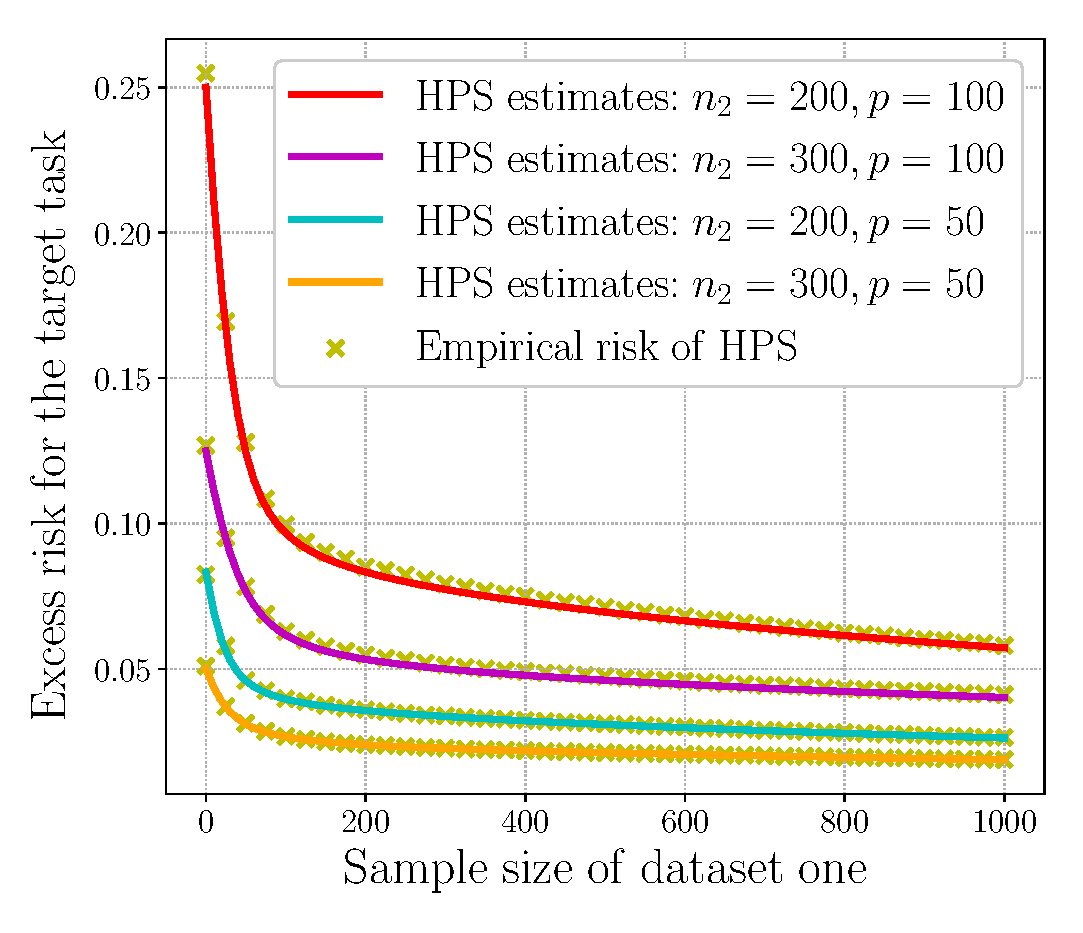
\includegraphics[width=0.8\textwidth]{figures/verify_covariate_shift.eps}
		\caption{Illustrating variance estimates for finite $p$}
		\label{fig_sec3_verify_cov}
	\end{subfigure}
	\begin{subfigure}[b]{0.5\textwidth}
		\centering
		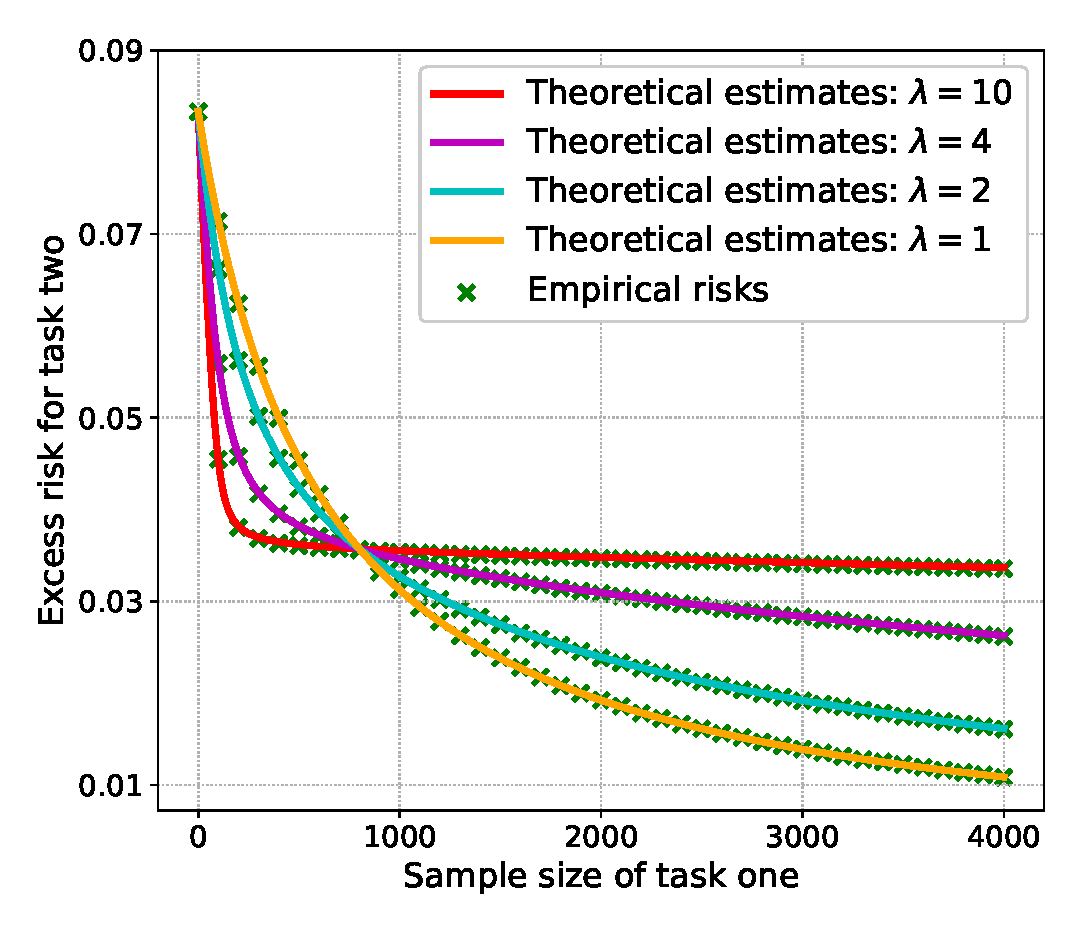
\includegraphics[width=0.8\textwidth]{figures/covariate_shift.eps}
		\caption{Varying the covariate shift parameter $\lambda$}
		\label{fig_sec3_covariate}
	\end{subfigure}
	\caption{We verify that Theorem \ref{thm_main_RMT} provides incredibly accurate estimates of the empirical variance under various finite sample sizes and dimensions.
	Furthermore, we illustrate an intriguing dichotomy between sample sizes and covariate (cf. Claim \ref{claim_dichotomy}).
	When $n_1 \ge n_2$, the lowest risk for predicting task two's labels is achieved by transferring from a dataset that has the same covariance matrix as task two. 
	When $n_1 < n_2$, the lowest risk is instead achieved by transferring a covariate-shifted dataset.
	Both simulation uses $\sigma = 1/2$.
	Figure \ref{fig_sec3_verify_cov} fixes $\lambda = 4$ and varies $n_1, p$.
	Figure \ref{fig_sec3_covariate} fixes $p = 100, n_2 = 300$ while varying $n_1, \lambda$.}
	\label{fig_sec31}
\end{figure}

\paragraph{Illustrative examples.} Next, we illustrate the result of Corollary \ref{cor_hps_cov} in several examples.
We use our estimates to explore whether covariate shift helps or hurts information transfer.
Our first example illustrates that the effect of covariate shift depends on the sample sizes of each dataset in an intricate manner.
    While the folklore belief is that transferring from a covariate-shifted distribution performs worse than an identical distribution, we show that, surprisingly, the former can sometimes outperform the latter.
    
    We first describe a setting for modeling covariate shift.
    Let $\cS$ be the set of positive definite matrices $M^{\top} M$ such that for $i = 1,2,\dots,\floor{\frac p 2}$, $\lambda_{p - i}  = \frac 1 {\lambda_i}$, where $\lambda_1 \ge \lambda_2 \ge \cdots \ge \lambda_p$ are the eigenvalues of $M$.
    Under this setting, we ask: suppose that the sample sizes $n_1$ and $n_2$ are both fixed, which $M$ provides the best ``transfer'' in the sense of HPS estimator's excess risk?
    We observe a dichotomy that depends on whether or not $n_1$ is greater than $n_2$.
    \begin{claim}[Sample sizes vs. covariate shift]\label{claim_dichotomy}
        Let $g(M) = \frac{\sigma^2}{n_1 + n_2} \bigtr{\frac 1 {\alpha_1 M^{\top} M + \alpha_2}}$.
        Suppose that $n_1$ and $n_2$ are both fixed.
        Within the set of all possible covariate shift matrix $M\in\cS$, the following dichotomy holds:
        \begin{enumerate}
	        \item[i)] If $n_1 \ge n_2$, then $g(M)$ is minimized in $\cS$ when $\lambda_i = 1$, for any $i = 1,\dots,p$.
	        \item[ii)] If $n_1 < n_2$, then $g(M)$ is maximized in $\cS$ when $\lambda_i = 1$, for any $i = 1,\dots,p$.
        \end{enumerate}
    \end{claim}

\begin{proof}
    For any $M \in \cS$, we can write $g(M)$ as
    $$g(M)=\frac{\sigma^2}{ n_1+n_2 }\sum_{i=1}^{p/2}\left( \frac{1}{\lambda_i^{2} \alpha_1 + \alpha_2} + \frac1{\lambda_i^{-2} \alpha_1 + \alpha_2} \right).$$
    When $M=\id_{p\times p}$, by the first equation of \eqref{eq_a12extra}, we have
    $$g(\id_{p\times p})=\frac{\sigma^2}{ n_1+n_2 }\sum_{i=1}^{p/2} \frac{2}{1-\gamma},$$
    where we abbreviate $\gamma:=p/(n_1+n_2)$.
    Using $\alpha_1 + \alpha_2 = 1-\gamma$, we further have that
    \begin{align*}
        g(M) - g(\id_{p\times p})%&= \frac{\sigma^2 \gamma}{2(1-\gamma)} (\lambda^2-1)a_1\cdot \bigbrace{  \frac{1}{ -a_1(\lambda^2-1)+(1-\gamma)\lambda^2 } - \frac{1}{a_1(\lambda^2-1) + (1-\gamma)}} \\
        &= \frac{\sigma^2 }{ n_1+n_2-p} \sum_{i=1}^{p/2} \frac{(\lambda_i^2-1)^2 \alpha_1 \left[ \alpha_1 - \alpha_2\right] }{[\alpha_1 + \lambda_i^2 \alpha_2][\lambda_i^2 \alpha_1 + \alpha_2]} .
    \end{align*}
    %in this example is equal to
    %$\frac{p}{2(n_1 + n_2)} f(\lambda)$, where
    %\[ f(\lambda) = {(\lambda^{-2} a_1 + a_2)^{-1} + (\lambda^2 a_1 + a_2)^{-1}}. \]
    %Using the fact that $a_1 + a_2 = 1 - \frac{p}{n_1 + n_2}$, we can verify
    %\begin{align*}
    %	f(\lambda) - f(1) &= \left(\lambda^2 a_1 + \frac{n_1 + n_2 - p}{n_1 + n_2} - a_1\right)^{-1} \\
    %	&+ \left(\lambda^{-2} a_1 + \frac{n_1 + n_2 - p}{n_1 + n_2} - a_1\right)^{-1} \\
    %	&- \frac{2(n_1 + n_2)}{n_1 + n_2 - p} \\
    %	&= \left(2a_1 - \frac{n_1 + n_2-p} {n_1 + n_2 }\right)  g(\lambda, a_1), %\cdot (\lambda^2-1)^2
    %\end{align*}
    %\begin{align*}
    %	f(\lambda) - f(1) &= \left(2a_1 - \frac{n_1 + n_2-p} {n_1 + n_2 }\right)  g(\lambda, a_1), %\cdot (\lambda^2-1)^2
    %\end{align*}
    %where $g(\lambda, a_1) \ge 0$.
    %and can be derived from algebraic calculations (details omitted).
    We claim that $\alpha_1 > \alpha_2$ if and only if $n_1 > n_2$, which proves claim i).
    In fact, if $\alpha_1 > \alpha_2$, then the first part of equation \eqref{eq_a12extra} gives that $\alpha_1 > (1-\gamma)/2$.
    The second part of equation \eqref{eq_a12extra} gives that
    \begin{align*}
     \frac{n_1}{n_1 + n_2} &> \alpha_1 + \frac{1}{n_1+n_2} \sum_{i=1}^{p/2}\left(\frac{\lambda_i^2}{\lambda_i^2+1}+\frac{\lambda_i^{-2}}{\lambda_i^{-2}+1}\right) = \frac{1-\gamma}{2}+\frac{\gamma}{2}=\frac{1}{2},
    \end{align*}
    %\begin{align*}
    % \frac{n_1}{n_1 + n_2} &=a_1 + \frac1{n_1 + n_2}\cdot \bigbrace{\sum_{i=1}^p \frac{\lambda_i^2 a_1}{\lambda_i^2 a_1 + a_2}} \\
    %	&> a_1 + \frac{p}{2(n_1+n_2)} \left(\frac{\lambda^2}{\lambda^2+1}+\frac{\lambda^{-2}}{\lambda^{-2}+1}\right) =\frac{1}{2}.
    %\end{align*}
    which is equivalent to $n_1>n_2$. The proof of claim ii) follows from a similar argument. % Similarly, if $a_1<a_2$, equations  \eqref{eq_a12extra000} and  \eqref{eq_a12extra} give that $a_1 < \frac{n_1 + n_2-p}{2 (n_1 + n_2)}$ and $n_1<n_2$. Thus, we conclude that $f(\lambda) \ge f(1)$ if and only if $n_1 \ge n_2$.
    %\end{example}
\end{proof}

Figure \ref{fig_sec3_covariate} illustrates a special case where $\lambda_1 = \cdots = \lambda_{\floor{p /2}} = \lambda > 0$ and the rest of the eigenvalues are all equal to $1 / \lambda$.
Thus, $\lambda > 0$ captures the degree of covariate shift: higher $\lambda$ implies worse covariate shift.
We observe that our theoretical estimates using Corollary \ref{cor_hps_cov} matches the empirical risks incredibly accurately.
As a result, we indeed observe the dichotomy shown in Claim \ref{claim_dichotomy}.
Furthermore, for higher $\lambda$, HPS' excess risk decreases slower--indicating a worse rate of ``transfer'' from task one. 
As a remark, the classical work of \citet{david2010impossibility} have likewise shown impossibility results for transfer learning under covariate shift in a classification setting.
By contrast, our analysis applies to a (high-dimensional) regression setting.


Our second example illustrates that the effect of covariate shift worsens as the sample size of task one increases.
We consider a set of covariate shift matrices $M^{\top} M$ whose determinant are all equal to one, and the eigenvalues are bounded between $\tau^2$ and $1 / \tau^2$.
Let $\cS$ denote the set of $M\in\real^{p\times p}$ such that $M^{\top} M$ satisfies both conditions.
\begin{claim}[Identical covariance provides approximately optimal transfer under imbalanced dataset sizes]\label{prop_covariate}
    Recall that $g(M) = \frac{\sigma^2}{n_1 + n_2} \bigtr{\frac 1 {\alpha_1 M^{\top} M + \alpha_2}}$.
	We have the following result regarding $g(\id_{p \times p})$:
	\begin{align} g(\id_{p\times p}) \le \bigbrace{1+ {\frac{n_2}{\tau^2 n_1}  }} g(M), \text{ for any } M \in \cS. \label{eq_claim_id}
	\end{align}
\end{claim}
\begin{proof}
    We can write the trace of $(\alpha_1 M^{\top} M + \alpha_2)^{-1}$ using the eigenvalues of $M^{\top} M$ as follows:
    \begin{align*}
        \bigtr{(\alpha_1 M^{\top} M + \alpha_2)^{-1}} &= \sum_{i=1}^p \frac{1} {\alpha_1 \lambda_i^2 + \alpha_2} \\
        &\ge \sum_{i=1}^p \frac{1} {\alpha_1 \lambda_i^2 + \alpha_2 \cdot {\lambda_i^2} / {\tau^2}} \tag{since $\lambda_i \ge \tau$, for any $i$} \\
        &= \frac 1 {\alpha_1 + \alpha_2 / \tau^2} \sum_{i=1}^ p \frac 1 {\lambda_i^2} \\
        &\ge \frac 1 {\alpha_1 + \alpha_2 /\tau^2} p\cdot \bigbrace{\prod_{i=1}^p \frac 1 {\lambda_i^2}}^{1/ p} \tag{by the AM-GM inequality} \\
        &= \frac{p}{\alpha_1 + \alpha_2 / \tau^2} \tag{since $\prod_{i=1}^p \lambda_i^2 = \det(M^{\top} M) = 1$}
    \end{align*}
    Next, recall from equation \eqref{g_id} that
    $g(\id_{p\times p}) = \frac{\sigma^2 p}{n_1 + n_2 - p}$.
    Thus, equation \eqref{eq_claim_id} follows if we show that (after rearranging terms)
    \begin{align}
        \frac{n_1 + n_2}{n_1 + n_2 - p} \cdot \frac 1 {\alpha_1 + \frac{\alpha_2}{\tau^2}} \le 1 + \frac{n_2}{\tau^2 \cdot n_1}. \label{eq_claim_id_step}
    \end{align}
    From the second part of equation \eqref{eq_a12extra}, we have that
    \begin{align*}
        \frac{n_1} {n_1 + n_2} &= \alpha_1 + \frac 1 {n_1 + n_2} \bigbrace{\sum_{i=1}^p \frac{\lambda_i^2\alpha_1}{\lambda_i^2\alpha_1 + \alpha_2}} \\
        &< \alpha_1 + \frac p {n_1 + n_2}.
    \end{align*}
    Thus, $\alpha_1 > \frac{n_1 - p}{n_1 + n_2}$, which implies that $\alpha_2 < \frac{n_2}{n_1 + n_2}$.
    Hence, $\alpha_1 + \frac{\alpha_2}{\tau^2} = 1 - \frac{p}{n_1 + n_2} - \alpha_2 + \frac{\alpha_2}{\tau^2} \le 1 - \frac{p}{n_1 + n_2} + \frac{n_2}{n_1 + n_2} \frac 1 {\tau^2}$, which implies
    equation \eqref{eq_claim_id_step} by straightforward calculations.
    Thus, the proof is complete.
\end{proof}
As a corollary of Claim \ref{prop_covariate}, when $n_1$ is much larger than $n_2 / \tau^2$, the excess risk of HPS is approximately optimal in the set of all possible $M\in\cS$ when there is no covariate shift between dataset one and two.





\subsection{Model shift}\label{sec_sizeratio}

Next, we consider a model shift setting where task one and two have the same linear model but different population covariance matrices.
We show the exact asymptotic limits of the bias and variance of HPS.

\begin{theorem}[Excess risk of HPS under model shift]\label{cor_MTL_loss}
Under Assumption \ref{assm_big1}, suppose that $\Sigma^{(1)}=\Sigma^{(2)}$ and the entries of $Z^{(1)}$ and $Z^{(2)}$ are i.i.d. Gaussian random variables.
Denote by $\xi_1:=p/n_1$ and $\xi_2:=p/n_2$.
Then, for any small constant $\e>0$ and large constant $C>0$, there exists a high probability event $\Xi$, on which the following estimates hold uniformly in all $a\in \R$:
\begin{align}
L_{\var}(a) &= \sigma^2  \cal L_1(a)+ \OO\Big(\frac {\sigma^2 p^{c}} {n_1}\Big), \label{Lvar_samplesize} \\
L_{\bias}(a)&= \bignorm{\beta^{(1)}-a\beta^{(2)}}^2 \cal L_2(a) +  \OO\Big(p^{-\frac 1 2 + c}  \norm{\beta^{(1)}-a\beta^{(2)}}^2
+ p^{-C}\big( \|\beta^{(1)} \|^2  +  \|\beta^{(2)} \|^2\big)   \Big),\label{Lbias_samplesize}
\end{align}
where $\cL_1(a)$ and $\cL_2(a)$ are defined as follows
\begin{align*}
\cal L_1(a) &:= {2p}\cdot\left((n_2 - p) + a^2 (n_1 - p) + \sqrt{\big( (n_2 - p) + a^2 (n_1 - p)\big)^2 + 4a^2(n_1 p + n_2 p - n_1 n_2)}\right)^{-1}, \\
\cal L_2(a) &:= \frac1{a^2}\cdot \frac{1- 2\frac{\cal L_1(a)}{\xi_2(1 + \cal L_1(a))} + \kappa(a)}{1- \xi_2 \kappa(a)}, \text{ in which }
\kappa(a) := \frac{\cal L_1(a)^2}{\xi_2^2(1+\cal L_1(a))^2}  \left(1 - \frac{a^4 \cal L_1(a)^2 }{\xi_1(1+a^2\cal L_1(a) )^2}\right)^{-1}.
%f_2(a):= \frac{a^4 \cal L_1(a)^2}{\xi_1^2 } \left[1 - \frac{a^4 \cal L_1(a)^2 }{\xi_1[1+a^2\cal L_1(a) ]^2}\right]^{-1},\\
%f_3(a):= \frac1{a^2}\frac{\xi_1}{\xi_2 +\cal L_1(a)}
 \end{align*}
%	In the setting of Example \ref{ex_sample_ratio}, assume that
%	%a) the sample sizes $n_1$ and $n_2$ are greater than $(1 + \tau) p$, b) $\Sigma_1=\Sigma_2=\id_p$, and c) %there exists a small constant $c_0>0$ such that
%	(i) both tasks sample sizes are at least $3p$;
%	(ii) noise variance is smaller than the shared signal variance: $\sigma^2 \lesssim  \kappa^2$;
%%	\be\label{choiceofpara0}
%%	p^{-1/2+c_0}\sigma^2 + p^{c_0}d^2\le \kappa^2\le p^{1-c_0} (\sigma^2 +d^2)  .  	\ee
%	%\be\label{choiceofpara0}
%%	(ii) the task-specific variance of $\beta_i$ is much smaller than the signal strength {\color{red}$d^2 = \oo( {\kappa^2})$}; \HZ{what does $\ll$ mean exactly?}
%%	(iii) the sample sizes $n_1$ and $n_2$ are greater than $(1 + \tau) p$.
%	(iii) task-specific variance is much smaller than the shared signal variance: $d^2 \le p^{-\e}{\kappa^2}$ for a small constant $c>0$.
%	Let $\varepsilon = (1 + \sqrt{p/n_1})^ 4 - 1$, which decreases as $n_1$ increases.
%	Let $\hat{A},\hat{B}$ be the global minimizer of $f(A, B)$.
%	With high probability over the randomness of the input,
%	the prediction loss of $\hat{\beta}_2^{\MTL} = \hat{B} \hat{A}_2$ for task two satisfies that
%	\begin{align}
%	%-\left[1- \left( 1-\frac{1}{\sqrt{\rho_1}}\right)^4\right] pd^2\cdot \frac{\rho_1^2 (\rho_1+\rho_2)}{(\rho_1 + \rho_2 - 1)^3} +\OO(p^{-c}\sigma^2)  \le
%	   \left|L(\hat{\beta}_2^{\MTL}) - \frac{2d^2 n_1^2 (n_1 + n_2)}{(n_1 + n_2 - p)^3} -\frac{\sigma^2 p}{n_1 + n_2 - p}  \right|
%	\le \varepsilon \cdot \frac{2d^2 n_1^2 (n_1 + n_2)}{(n_1 + n_2 - p)^3} +  \OO(p^{-c/2}).\label{cor_MTL_error}
%	%\left[\left( 1+\frac{1}{\sqrt{\rho_1}}\right)^4-1\right] d^2\cdot \frac{\rho_1^2 (\rho_1+\rho_2)}{(\rho_1 + \rho_2 - 1)^3} \\
%	%& +C \left[(p^{-c_\varphi}+p^{-c_\infty/2})(\sigma^2 +d^2)+p^{-c_\infty}\kappa^2 + %\frac{d^4+\sigma^2 d^2}{\kappa^2}\right],\nonumber
%	 \end{align}
%	 with high probability for any fixed $c\in(0, \min(\frac{1}{4}, \delta,\frac{\varphi-4}{2\varphi}))$.
%	 {\color{red}[FY: the error also contains $p^{-1/2+2c}\kappa^2 +  p^{-1/4+c} (\sigma^2 +d^2) $, both of which cannot be omitted, because (i) there is no assumption on the upper bound of $\kappa^2$, and (ii) we do not necessarily have $c_\varphi<1/4$. We can decide how to present the result concisely (for instance we can impose an upper bound on $\kappa^2$ and that $c_\varphi<1/4$), but it needs to be correct.]}
	 \end{theorem}

\iffalse
 We need to state a result for Gaussian matrix ...... Consider
$$f (\al,n_1,n_2)= \frac1p\tr\left[\frac{1}{ (X_1^\top X_1 + \al \cdot X_2^\top X_2)^2} (X_1^\top X_1)^2\right].$$
In our case, we have $\al=1$, but we can handle more general $\al$. We introduce two parameters:
$$a= \al \frac{n_2}{n_1} \left( \frac{p}{n_1} + \frac{p}{n_2}- \frac{p}{n_1 }\cdot \frac{p}{n_2}\right),\quad b= \al \frac{n_2}{n_1}\left( 1- \frac{p}{n_2}\right) + \left( 1- \frac{p}{n_1}\right). $$
Then we define the following parameters:
\begin{align*}
x= \frac{-b+ \sqrt{b^2 + 4a}}{2a},\quad y= \left[ x^{-2} - \frac{p}{n_1}\left( 1+\frac{p}{n_1}x\right)^{-2}\right]^{-1},\quad \omega= \al\frac{n_2}{n_1} \left( 1 + \al \frac{p}{n_1}x\right)^{-1}.
\end{align*}
We have that
$$f(\al,n_1,n_2)= \frac{1 - 2\omega x + \omega^2 y}{ 1 - \frac{p}{n_2} \cdot \omega^2 y } +\oo(1)\quad \text{w.h.p.} $$
In the setting $\al=1$, both $\omega x$ and $\omega^2 y$ can be written in terms of only one parameter
%$$f(\al,n_1,n_2)= \frac{\left(u^2 -\frac{p}{n_1}\right) \left(1- 2\frac{n_2}{n_1}  u^{-1}\right) + \frac{n_2^2}{n_1^2} }{ u^2 -\frac{p}{n_1}\left(1 + \frac{n_2}{n_1}\right) } +\oo(1)\quad \text{w.h.p.} $$
%where
$$u: = x^{-1}\left(1+\frac{p}{n_1}x\right)=   \frac{ b+\sqrt{b^2+4a}}{2} +\frac{p}{n_1}   .$$
\fi

Combining equation \eqref{Lvar_samplesize} and \eqref{Lbias_samplesize}, we thus obtain an estimate for the excess risk of HPS.
We provide some intuition behind both estimates.
%For the variance estimate in \eqref{Lvar_samplesize}, it is not necessary to assume the Gaussian distributions of the $Z^{(1)}$ and $Z^{(2)}$ entries.
First, the variance estimate is a special case of Theorem \ref{thm_main_RMT} where $\Sigma^{(1)} = \Sigma^{(2)}$ but $n_1 \neq n_2$.
In fact, the result can be obtained by solving $\alpha_1, \alpha_2$ in equation \eqref{eq_a12extra} using $\lambda_i = 1$ for all $i = 1,\dots, p$.
%On the other hand, the Gaussian assumption is needed in our current proof of the bias limit \eqref{Lbias_samplesize}.
Second, the bias estimate is obtained based on a sharp convergence estimate proved in \citet{BES_free1,BES_free2} for the free addition of two probability measures.
To illustrate, denote by $\bv(a):=(\Sigma^{(1)})^{1/2}\left(a\beta^{(1)}- a^2\beta^{(2)}\right)$.
We can write the bias equation as
\begin{align*}
    L_{\bias} (a)&=\bv_a^\top (Z^{(1)})^\top Z^{(1)} { \left(a^2(Z^{(1)})^\top Z^{(1)}+ (Z^{(2)})^\top Z^{(2)}  \right)^{-2}}(Z^{(1)})^\top Z^{(1)} \bv_a,
\end{align*}
By the rotational invariance of $(Z^{(1)})^\top Z^{(1)}$ and $(Z^{(2)})^\top Z^{(2)}$, we have that
\begin{align}\label{Lbias_idea}
    L_{\bias} (a)&\approx \|\bv_a\|^2 \cdot \frac1p\bigtr{ \big((Z^{(1)})^\top Z^{(1)}\big)^2 { \left(a^2(Z^{(1)})^\top Z^{(1)}+ (Z^{(2)})^\top Z^{(2)}\right)^{-2}}}
\end{align}
up to a small error.

Our key idea is to write equation \eqref{Lbias_idea} as the derivative of a certain polynomial with respect to $x$ at $x = 0$:
\begin{align}\nonumber %\label{Lbias_idea2}
L_{\bias} (a)&\approx \|\bv_a\|^2 \cdot\left. \frac{\dd }{\dd x}\right|_{x=0}\frac1p\bigtr{  \Big( a^2(Z^{(1)})^\top Z^{(1)} + x \big((Z^{(1)})^\top Z^{(1)}\big)^2 + (Z^{(2)})^\top Z^{(2)} \Big)^{-1}  }.
\end{align}
It is well-known that the empirical spectral distributions (ESD) of $(Z^{(i)})^\top Z^{(i)}$, $i=1,2$, satisfy the famous Marchenko-Pastur (MP) law asymptotically \cite{MP}. From the MP law of $(Z^{(1)})^\top Z^{(1)}$, we can also derive the asymptotic ESD of $a^2(Z^{(1)})^\top Z^{(1)}+ x[(Z^{(1)})^\top Z^{(1)}]^2$ for any fixed $a\in \R$ and $x>0$. Due to the rotational invariance of multivariate Gaussian distributions,
%$a^2(Z^{(1)})^\top Z^{(1)}+ x[(Z^{(1)})^\top Z^{(1)}]^2$ and $(Z^{(2)})^\top Z^{(2)}$ are asymptotically freely independent from each other \cite{nica2006lectures}. Hence
the asymptotic ESD of $a^2(Z^{(1)})^\top Z^{(1)}+ x[(Z^{(1)})^\top Z^{(1)}]^2+(Z^{(2)})^\top Z^{(2)}$ is given by the free additive convolution (or free addition) of the asymptotic ESD of $a^2(Z^{(1)})^\top Z^{(1)}+ x[(Z^{(1)})^\top Z^{(1)}]^2$ and the MP law of $(Z^{(2)})^\top Z^{(2)}$\cite{nica2006lectures}.
%In particular, a sharp convergence estimate has been proved in \cite{BES_free1,BES_free2} for the free addition of two probability measures.
Finally, We use the result of \citet{BES_free1,BES_free2} to obtain a sharp estimate of
$$\frac1p\bigtr{  \Big( a^2(Z^{(1)})^\top Z^{(1)}+ x \big((Z^{(1)})^\top Z^{(1)}\big)^2+(Z^{(2)})^\top Z^{(2)} \Big)^{-1}},$$
which implies a sharp estimate of $L_{\bias}(a)$.
%Taking the derivative with respect to $x$ at $x=0$ gives the exact asymptotic limit of $L_{\bias}(a)$.
\todo{can we add a few sentences to describe any technical challenge here? right now it sounds like our result is a direct corollary, which is not good?}
The complete proof of Theorem \ref{cor_MTL_loss} can be found in Section \ref{app_iso_cov}.

\medskip
\noindent\textit{Remarks.}
First, we believe the convergence rates $p^c/n_1$ and $p^{-1/2+c}$ in \eqref{Lvar_samplesize} and \eqref{Lbias_samplesize} are both sharp up to the $p^c$ factor.
\todo{the rate in \eqref{Lvar_samplesize} seems different from Thm 3.1?}
Second, we believe that the above argument can be extended to the case without the Gaussian assumption. For example, instead of using the results in \cite{BES_free1,BES_free2} on free addition, we can use the sharp local laws on polynomials of random matrices in \cite{EKN_poly}. However, applying the result of \citet{EKN_poly} requires checking certain technical regularity conditions for our setting. We leave this as an open question for future work.

\begin{figure}[!t]
	\begin{subfigure}[b]{0.33\textwidth}
		\centering
		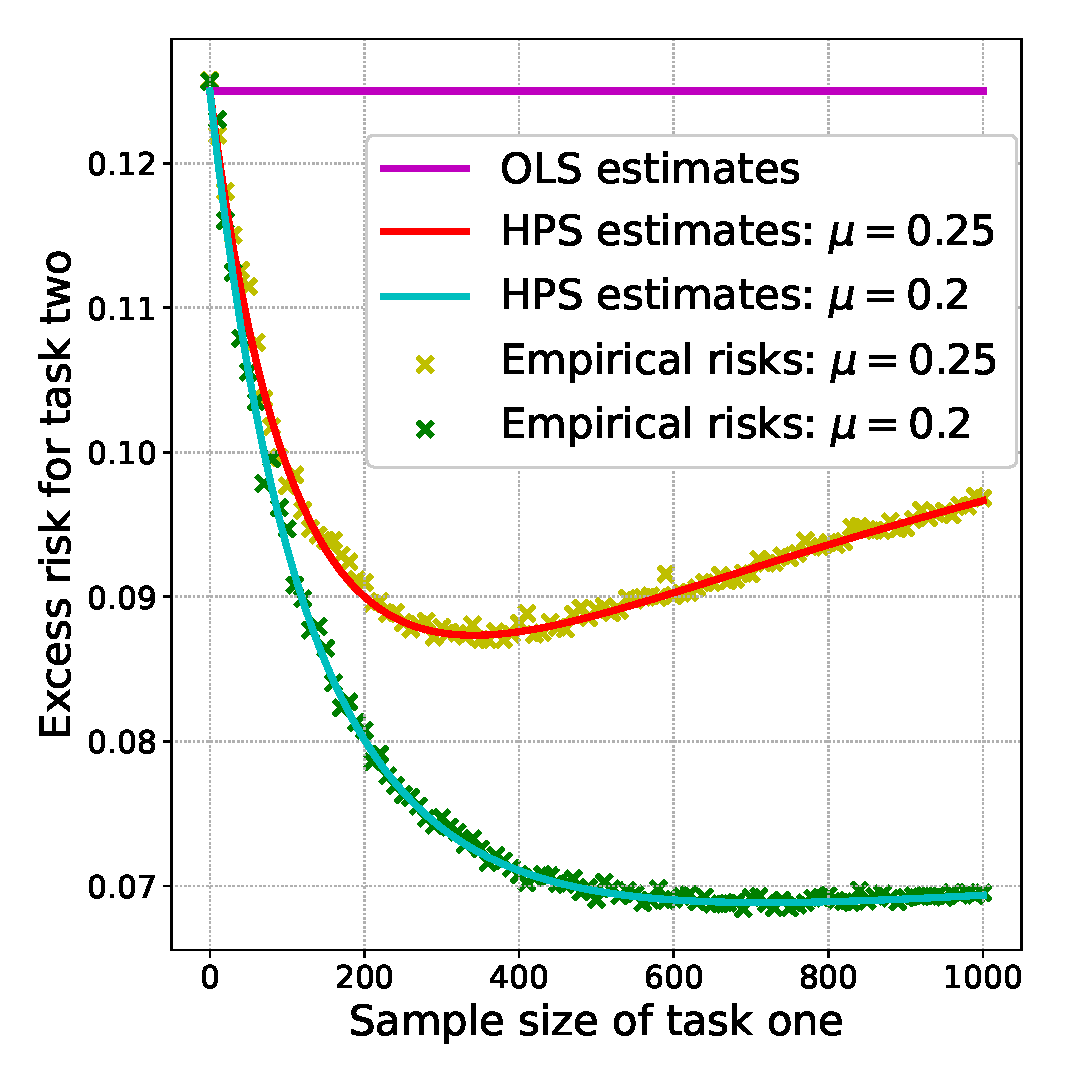
\includegraphics[width=0.95\textwidth]{figures/model_shift_positive.eps}
		\caption{Positive transfer}
		\label{fig_sec3_model_positive}
	\end{subfigure}\hfill%
	\begin{subfigure}[b]{0.33\textwidth}
		\centering
		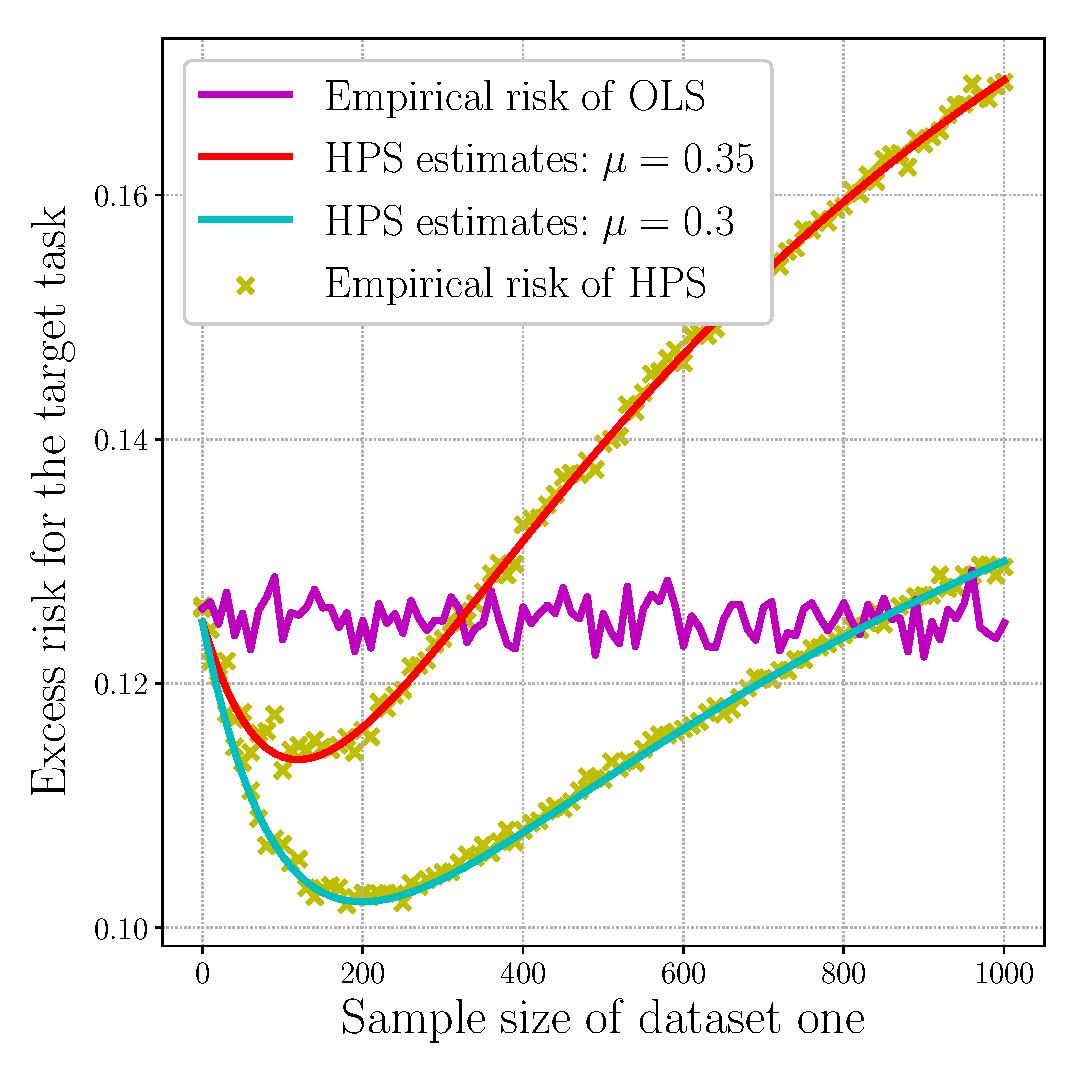
\includegraphics[width=0.95\textwidth]{figures/model_shift_transition.eps}
		\caption{From positive to negative transfer}
		\label{fig_sec3_model_transition}
	\end{subfigure}\hfill%
	\begin{subfigure}[b]{0.33\textwidth}
		\centering
		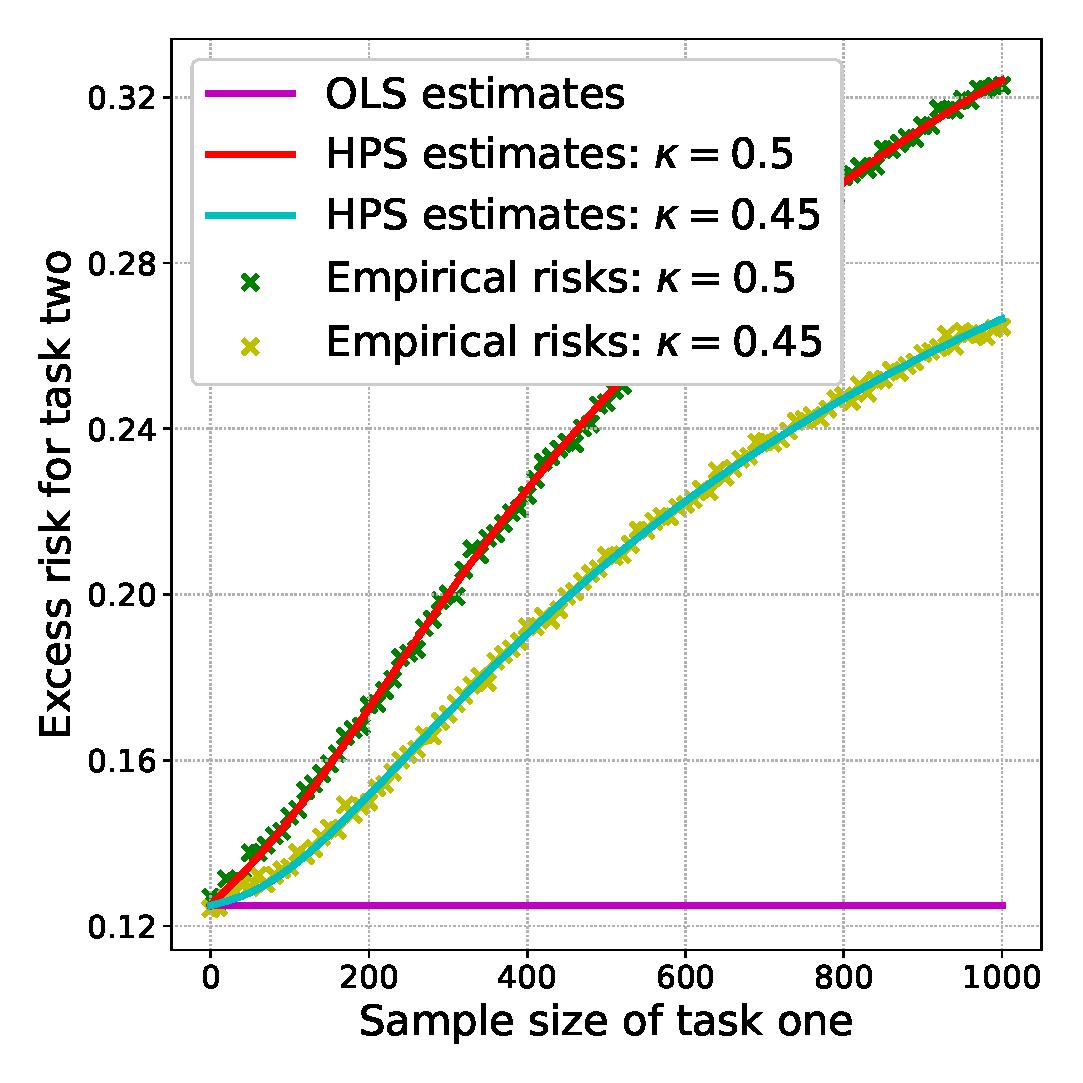
\includegraphics[width=0.95\textwidth]{figures/model_shift_negative.eps}
		\caption{Negative transfer}
		\label{fig_sec3_model_negative}
	\end{subfigure}	
	\caption{We illustrate three regimes of information transfer in HPS under model shift. When $\mu$ is small, HPS outperforms the OLS estimator irrespective of $n_1$. When $\mu$ is large, HPS performs worse than OLS. For an intermediate range of $\mu$, HPS outperforms OLS only for a restricted range of $n_1$. See Claim \ref{claim_model_shift} for the precise range of each regime. This simulation fixes $p = 100, n_2 = 300, \sigma = 1/2$ while varying $n_1, \mu$.}
	\label{fig_sec3_model_shift}
\end{figure}

\paragraph{Illustrative examples.}
While the estimates from Theorem \ref{cor_MTL_loss} are generally complex, we describe a simplified result for the random-effect model (cf. Section \ref{sec_data}).
Under the assumptions stated in Proposition \ref{lem_hat_v}, $\hat{a}$ is approximately equal to one.
Then, we can calculate that
\[ \cL_1(1) = \frac{p}{n_1 + n_2 - p} \text{ and } \cL_2(1) = \frac{n_1^2(n_1 + n_2 - p) + p n_1 n_2}{(n_1 + n_2)^2 (n_1 + n_2 - p)}, \text{ in which } \kappa(1) = \frac{n_2^2}{(n_1 + n_2)^2 - n_1 p}. \]
Thus, using that $\|\beta^{(1)}-\beta^{(2)}\|^2 = (2+\oo(1))\mu^2$ w.h.p., we conclude that for the random-effect model, the excess risk $L(\hat{\beta}_2^{\MTL})$ is approximately equal to
$$ g(n_1) \define \sigma^2 \cal L_1(1) +   2\mu^2 \cal L_2(1)= \frac{p\sigma^2}{n_1+n_2-p} +  2\mu^2 \cdot \frac{n_1^2 (n_1+n_2-p)+p n_1n_2}{(n_1+n_2)^2(n_1+n_2-p)}$$
plus lower order terms (that vanishes to zero as $p$ goes to infinity).
Next, we analyze when combining task one using HPS transfers positively to task two, depending on sample sizes $n_1, n_2$, and the model shift parameter $\mu$ in the random-effect model.

\begin{claim}[Sample sizes vs. model shift]\label{claim_model_shift}
    Suppose Assumption \ref{assm_big1} and the random-effect model under equation \eqref{eq_re} and \eqref{para_rel} holds.
    Suppose further that $n_2 \ge 3p$.
    Then, there exists a large constant $C > 0$ such that the following holds w.h.p.,
    \begin{enumerate}
        \item[i)] If $\mu^2 \le \frac{\sigma^2 p}{2(n_2 - p)}$, then $L(\hat{\beta}_2^{\MTL}) \le L(\hat{\beta}_2^{\STL}) + \OO(p^{-C})$.
        \item[ii)] If $\frac{\sigma^2 p}{2(n_2 - p)} < \mu^2 < \frac{\sigma^2 n_2}{2(n_2 - p)}$, then there exists a deterministic constant $\rho$ such that if $n_1 \le \rho\cdot p$, then $L(\hat{\beta}_2^{\MTL}) \le L(\hat{\beta}_2^{\STL}) + \OO(p^{-C})$, else $L(\hat{\beta}_2^{\STL}) \le L(\hat{\beta}_2^{\MTL}) + \OO(p^{-C})$.
        \item[iii)] If $\frac{\sigma^2 n_2} {2(n_2 - p)} \le \mu^2$, then $L(\hat{\beta}_2^{\STL}) \le L(\hat{\beta}_2^{\MTL}) + \OO(p^{-C})$.
    \end{enumerate}
\end{claim}

\begin{proof}
By Theorem \ref{cor_MTL_loss} and the discussion above, we have that $L(\hat{\beta}_2^{\MTL}) = g(n) + \OO(p^{-C})$ w.h.p.
By Lemma \ref{fact_tr}, we have that the excess risk of the OLS estimator for task two satisfies
\begin{align*}
    L(\hat{\beta}_2^{\STL})
    = \sigma^2 \cdot \bigtr{\Sigma^{(2)}\Big((X^{(2)})^{\top} X^{(2)} \Big)^{-1}}
    = \frac{\sigma^2 p}{n_2 - p} + \OO(p^{-C}).
\end{align*}
Thus, whether or not $L(\hat{\beta}_2^{\MTL}) \le L(\hat{\beta}_2^{\STL})$ reduces to comparing $g(n_1)$ and $\frac{\sigma^2 p}{n_2 - p}$---let $h(n_1)$ be their difference.
We can write $h(n_1)$ as
\[ h(n_1) = 2\mu^2 \cdot \frac{n_1^2 (n_1 + n_2 - p) + p n_1 n_2}{(n_1 + n_2)^2 (n_1 + n_2 - p)} - \frac{\sigma^2 p n_1}{(n_1 + n_2 - p)(n_2 - p)}. \]
We observe that the sign of $h(n_1)$ is the same as the sign of the following simplified polynomial
\begin{align*}
    \tilde h(n_1) &= 2\mu^2 (n_2 - p) (n_1 (n_1 + n_2 - p) + p n_2) - \sigma^2 (n_1 + n_2)^2 \\
    &= \big(2\mu^2 (n_2 - p) - \sigma^2\big) n_1^2 + (2\mu^2 (n_2 - p)^2 - 2\sigma^2 p n_2) n_1 + \big(2\mu^2 (n_2 - p) p n_2 - \sigma^2 p n_2^2\big).
\end{align*}
Let $C_0, C_1, C_2$ be the coefficient of $n_1^0, n_1^1, n_1^2$ above, respectively.
We argue about each claim as follows.

For claim i), if $\mu^2 \le \frac{\sigma^2 p}{2(n_2 - p)}$, then $C_0, C_1, C_2$ are all at most zero.
Thus, $\tilde h(n_1) \le 0$, which implies that $h(n_1) \le 0$.

For claim ii), if $\frac{\sigma^2 p}{2(n_2 - p)}< \mu^2 < \frac{\sigma^2 n_2}{2(n_2 - p)}$ (recall that $n_2 > p$ by Assumption \ref{assm_big1}), then $C_2 > 0$ and $C_0 < 0$.
Thus, $\tilde{h}(n_1)$ has a positive root and a negative root.
Let $\rho$ be the positive root.
Hence, if $n_1 \le \rho \cdot p$, then $\tilde h(n_1) \le 0$.
Otherwise, $\tilde h(n_1) \ge 0$.

For claim iii), if $\frac{\sigma^2 n_2}{2(n_2 - p)} \le \mu^2$, then $C_1 \ge 0$ and $C_2 \ge 0$.
Furthermore, $\frac{\sigma^2 p n_2}{(n_2 - p)^2} \le \frac{\sigma^2 n_2}{2(n_2 - p)}$ because $n_2 \ge 3p$ by our assumption.
Thus, $C_2$ is non-negative as well, which implies $\tilde h(n_1) \ge 0$.
\end{proof}

As a remark, when $p < n_2 < 3p$, similar results can be derived using the above arguments (details omitted).
Figure \ref{fig_sec3_model_shift} illustrates Claim \ref{claim_model_shift} for different regimes of model shift parameter $\mu$ in the random-effect model.
This simulation affirms that our estimates accurately match with the empirical bias equation \eqref{Lbias} plus the variance equation \eqref{Lvar}.
Furthermore, we observe the three information transfer regimes shown in Claim \ref{claim_model_shift} by varying $\mu$ in the random-effect model.





\subsection{Covariate and model shift}\label{sec3_combined}


For the bias limit, we have the following proposition.

\begin{theorem}[Bias estimates under covariate and model shift]\label{prop_main_RMT}
%The bias equation \eqref{Lbias} satisfies the following limit with high probability: Let $S$ be an arbitrary subset of the unit sphere in dimension $p$ whose size is polynomial in $p$, for any unit vector $w\in S$,
Under Assumption \ref{assm_big1}, for any small constant $c>0$ and large constant $C>0$, there exists a high probability event $\Xi$, on which the following estimate  holds for $L_{\bias}(a)$ in \eqref{Lbias}:
			\begin{align}
				& \bigabs{ L_{\bias}(a) -   (\beta^{(1)}- a\beta^{(2)} )^\top (\Sigma^{(1)})^{1/2} \Pi(a)(\Sigma^{(1)})^{1/2} (\beta^{(1)}- a\beta^{(2)})   }  \nonumber\\
				& \le \left[\left( 1+\sqrt{\frac{p}{n_1}}\right)^4 - 1 +\OO\left( n_1^{-1/2+2/\varphi + c}\right)\right] \frac{n_1^2 \lambda_1^2 \left\|(\Sigma^{(1)})^{1/2} \left(\beta^{(1)}- a\beta^{(2)}\right) \right\|^2}{  [(\sqrt{n_1}-\sqrt{p})^2 \lambda_p^2+ (\sqrt{n_2}-\sqrt{p})^2]^2}  \nonumber\\
				& + p^{-C} \left[\| \beta^{(1)}\|^2 + \| \beta^{(2)}\|^2 \right], \label{lem_cov_derv_eq}
			\end{align}
%			\begin{align}\label{lem_cov_derv_eq}
%				\bigabs{ L_{\bias}(a) - \left\|\frac{n_1}{n_1+n_2}  \frac{\left[a_3 M(a)^\top M(a) + (a_4 + 1) \right]^{1/2}}{ a_1 M(a)^\top M(a) + a_2 } M(a)^\top (\Sigma^{(1)})^{1/2} \left(\beta^{(1)}- a\beta^{(2)}\right)\right\|^2   } \le  \frac{p^{-c_{\varphi}}}{(n_1+n_2)^2},
%			\end{align}
				uniformly in all $a\in \R$. Here $\lambda_1$ and $\lambda_p$ are respectively the largest and smallest singular values of $M(a)$, $\Pi(a)$ is a $p\times p$ matrix defined as
				$$\Pi(a):=\frac{n_1^2}{(n_1+n_2)^2}  M(a)  \frac{a_3 M(a)^\top M(a) + (a_4 + 1) }{[a_1 M(a)^\top M(a) + a_2 ]^2} M(a)^\top  ,$$
				 and $(a_{3},a_4)$ is the solution of the following system of equations % with $b_k = \frac1{p}\sum_{i=1}^p \frac{\lambda_i^{2k}} {(\lambda_i^2 a_1 + a_2)^2}$, for $k = 0, 1, 2$:
		\be  \label{eq_a34extra}
		\begin{split}
				& a_3 + a_4 = \frac{1}{n_1 + n_2}\sum_{i=1}^p \frac{1}{\lambda_i^2 a_1 + a_2}, \\
				& a_3 + \frac{1}{n_1 + n_2} \sum_{i=1}^p \frac{\lambda_i^2 (a_2 a_3-a_1 a_4 )}{(\lambda_i^2 a_1 + a_2)^2} = \frac{1}{n_1 + n_2} \sum_{i=1}^p \frac{\lambda_i^2 a_1}{(\lambda_i^2 a_1 + a_2)^{2}},
%				\left(\frac{\rho_1}{a_1^{2}} -  b_2  \right)\cdot  a_3 -  b_1 \cdot  a_4 = b_1,\quad \left(\frac{\rho_2}{a_2^{2}}-  b_0\right)\cdot  a_4 - b_1 \cdot  a_3
%				= b_0.
			\end{split}
			\ee
			where we recall that $(a_1,a_2)$ is the solution of \eqref{eq_a12extra}.
\end{theorem}

Note that the first error term on the right-hand side of \eqref{lem_cov_derv_eq} is typically smaller than the main term $ (\beta^{(1)}- a\beta^{(2)} )^\top (\Sigma^{(1)})^{1/2} \Pi(a)(\Sigma^{(1)})^{1/2} (\beta^{(1)}- a\beta^{(2)})  $ by a factor of $\OO(\sqrt{p/n_1} + n_1^{-1/2+2/\varphi + c})$. Hence \eqref{lem_cov_derv_eq} only gives an exact asymptotic limit in the regime $n_1\gg p$. Moreover, by equations \eqref{eq_a12extra} and \eqref{eq_a34extra} we have
$$a_1 =\frac{n_1}{n_1+n_2} + \OO\left( \frac{p}{n_1+n_2}\right), \quad a_3 =\frac{n_3}{n_1+n_2} + \OO\left( \frac{p}{n_1+n_2}\right),$$
and
$$a_3 =\OO\left( \frac{p}{n_1+n_2}\right),\quad a_4 =\OO\left( \frac{p}{n_1+n_2}\right).$$
Using these estimates, it is easy to check that
\begin{align}
& (\beta^{(1)}- a\beta^{(2)} )^\top (\Sigma^{(1)})^{1/2} \Pi(a)(\Sigma^{(1)})^{1/2} (\beta^{(1)}- a\beta^{(2)})   \nonumber \\
&=\left\| (\Sigma^{(2)})^{1/2}\frac{1}{a^2\Sigma^{(1)}+\Sigma^{(2)}} a \Sigma^{(1)} \left(\beta^{(1)}- a\beta^{(2)}\right) \right\|^2 + \OO\left( \frac{p\left\|\beta^{(1)}- a\beta^{(2)}\right\|^2}{n_1+n_2}  \right)  . \label{bias_LLN}
\end{align}
Hence \eqref{lem_cov_derv_eq} is consistent with the result obtained by replacing $ (X^{(1)})^\top X^{(1)}$ and $ (X^{(2)})^\top X^{(2)}$ with $n_1\Sigma^{(1)}$ and $n_2\Sigma^{(2)}$, respectively, in $L_{\bias} (a) $ using the law of large numbers in the regime $n_1\gg p$. However, simulations show that our estimate \eqref{lem_cov_derv_eq} is more precise than the first term on the right-hand side of \eqref{bias_LLN}.

\begin{remark}
%First, our result in Corollary \ref{cor_MTL_loss} involves an error term that scales down with $n_1$.
%Tightening this error bound requires showing the limit of $\normFro{({Z^{(1)}}^{\top} Z^{(1)} + {Z^{(2)}}^{\top} Z^{(2)})^{-1} {Z^{(1)}}^{\top} Z^{(1)}}^2$ for two isotropic sample covariance matrices.
%This requires studying the asymptotic singular values distribution of the non-symmetric matrix $({Z^{(1)}}^{\top} Z^{(1)})^{-1}{Z^{(2)}}^{\top} Z^{(2)}+\id$, which is still an open problem in random matrix theory.
%\begin{remark}
The main error in Proposition \ref{prop_main_RMT} comes from approximating $(Z^{(1)})^\top Z^{(1)}$ by $n_1\id_{n_1\times n_2}$ using Corollary \ref{fact_minv} in the supplement \cite{MTL_suppl}. In order to improve this estimate and obtain an exact asymptotic result, one needs to study the singular value distribution of the  random matrix $\cal X + a^2$ for any fixed $a\in \R$, where $\cal X:=[(X^{(1)})^{\top}X^{(1)}]^{-1}(X^{(2)})^{\top}X^{(2)}$. We remark that the eigenvalues of $\cal X$ have been studied in the name of Fisher matrices \cite{Fmatrix}. However, since $\cal X$ is not symmetric, its singular values are different from its eigenvalues. To the best of our knowledge, the asymptotic singular value behavior of $\cal X$ is still an open problem in random matrix theory, and the study of the singular values of $\cal X + a^2$ will be even harder. We leave this problem to future study.

We also remark for the general case with covariate shift, the method in Section \ref{sec_sizeratio} for the bias term also fails, because we cannot reduce the problem into the free addition of two random matrices that are asymptotically freely independent.
%\end{remark}
\end{remark}

\begin{figure}[!t]
	\begin{subfigure}[b]{0.5\textwidth}
		\centering
		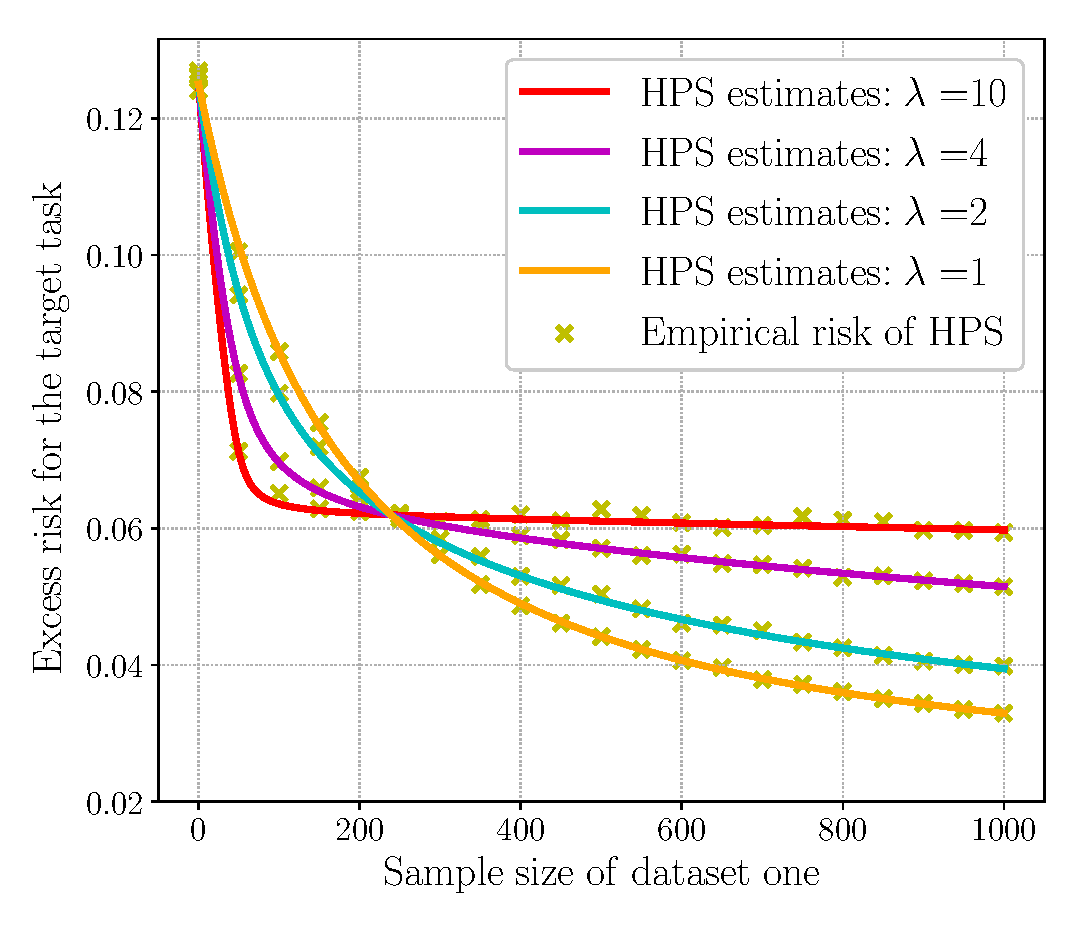
\includegraphics[width=0.8\textwidth]{figures/covariate_and_model_shift_a.eps}
		\caption{Fixed $\mu$, different $\lambda$}
		\label{fig_sec3_cov_mo_a}
	\end{subfigure}
	\begin{subfigure}[b]{0.5\textwidth}
		\centering
		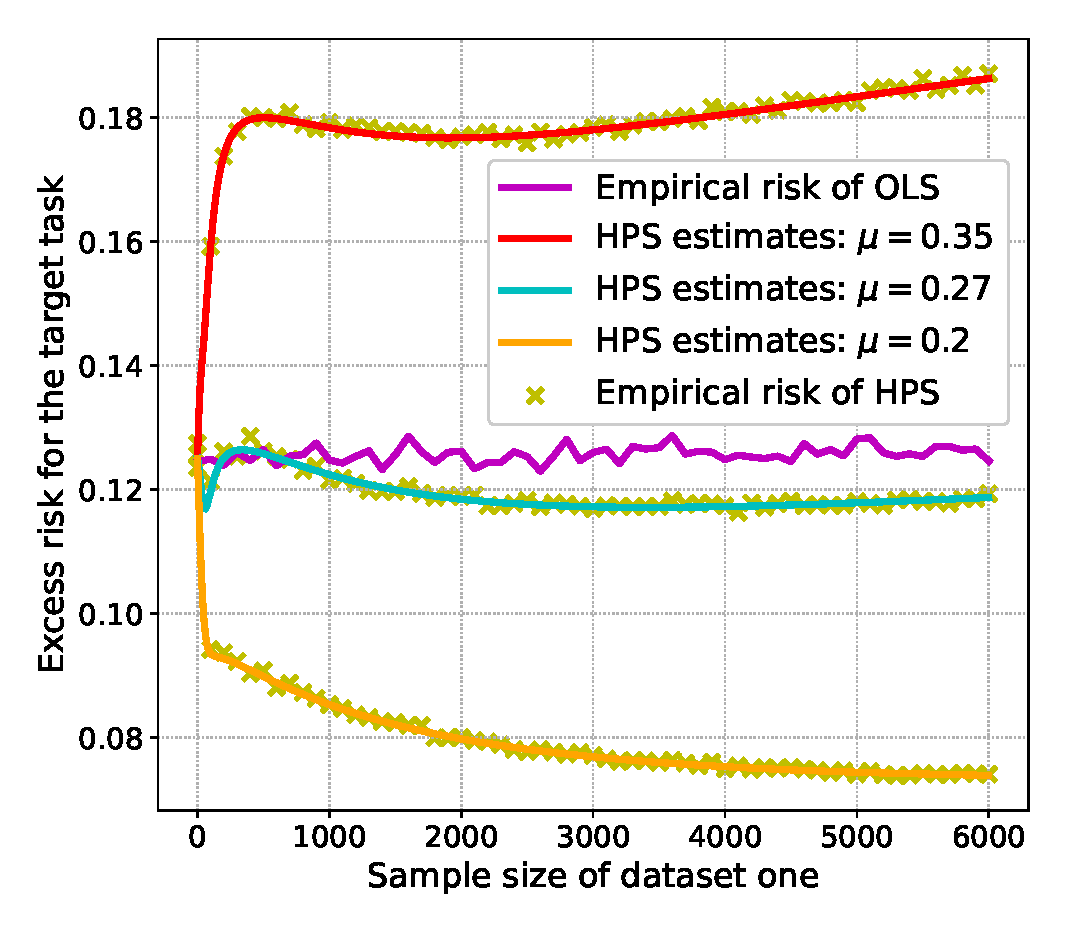
\includegraphics[width=0.8\textwidth]{figures/covariate_and_model_shift_b.eps}
		\caption{Fixed $\lambda$, different $\mu$}
		\label{fig_sec3_cov_mo_b}
	\end{subfigure}
	\caption{We further show that our observations in Figures \ref{fig_sec31} and \ref{fig_sec3_model_shift} extend to settings with both covariate and model shift.
	Both simulation use $p = 100, n_2 = 300, \sigma = 1/2$.
	Figure \ref{fig_sec3_cov_mo_a} fixes $\mu = 0.1$ while varying $\lambda, n_1$.
	Figure \ref{fig_sec3_cov_mo_b} fixes $\lambda = 4$ while varying $\mu, n_1$.}
	\label{fig_sec33}
\end{figure}

Consider the special case with $\Sigma^{(2)}=\id$, $a=1$ and the random effect model. Let $\sigma_i^{(1)}$ be the eigenvalues of $\Sigma^{(1)}$. Define the function 
\be\label{g1new} g_0(x)= \frac{1}{n_1}\sum_{i=1}^p \frac{\sigma_i^{(1)}}{1+ \sigma_i^{(1)} x} -\frac{1}{x} .\ee
Let $y$ be the unique positive solution to the equation 
\be\nonumber
\frac{n_1+n_2-p}{n_1} + g_0(y) \cdot \left( 1+    y\right)=0 .
\ee
Define the following three functions of $y$:
$$f_1= \frac{n_1}{p}y + \frac{n_1-p}{p}\frac1{g_0(y)},\quad f_2= \frac{n_1}{p}\frac{1}{g_0'(y)}- \frac{n_1-p}{p}\frac1{[g_0(y)]^2},\quad f_3= - g_0(y),$$
where $g_0'(y)$ is the derivative
$$ g_0'(y)=  -\frac{1}{n_1}\sum_{i=1}^p \frac{(\sigma_i^{(1)})^2}{(1+ \sigma_i^{(1)} y)^2} +\frac{1}{y^2}. $$
Then the variance limit is given by
$$ L_{\var}(1)=\sigma^2 \frac{p}{n_1}f_1,$$
and the bias limit is given by 
$$ L_{\bias}(1)=2\mu^2 \frac{1 - 2f_1 f_3  +f_2 f_3^2  }{ 1 - \frac{p}{n_2}f_2 f_3^2 }.$$
(Here $2\mu^2$ represents $\|\beta^{(1)}-\beta^{(2)}\|^2$.)

    \section{Extension to multiple data sources}\label{sec_same}

Our setup and the results in Section \ref{sec_main} are both for transferring from one data source.
This section extends our setup to transfer learning from multiple data sources.
We focus on a natural setting where all the tasks have the same covariates but different labels.

\paragraph{Data model.} Suppose we have $t$ datasets whose sample sizes are all equal to $n$ and whose feature covariates are all equal to $X \in \real^{n \times p}$. The label vector of the $i$-th task follows a linear model
\begin{align}\label{eq_mtl_data}
    Y^{(i)} = X \beta^{(i)} + \varepsilon^{(i)}, \text{ for } i=1, 2,\cdots, t.
\end{align}
Similar to Section \ref{sec_main}, we use the first $(t-1)$ datasets as sources to predict the $t$-th task.
However, there is a \text{model shift} between the data sources and the task we would like to predict.
We make several standard assumptions on $X$ and each of $\varepsilon^{(i)}$.
First, $X = Z\Sigma^{1/2}$ is a random matrix satisfying Assumption \ref{assm_big1} (same as $X^{(2)}$).
In particular, the sample size $n$ is greater than the dimension $p$.
Second, every $\varepsilon^{(i)} \in \real^{n}$ is a random vector with i.i.d entries of mean zero, variance $\sigma^2$, and bounded moments up to any order (cf. equation \eqref{eq_highmoments}).
Finally, $\beta^{(i)} \in \real^{p}$ is a fixed vector independent from any other $\beta^{(j)}$ for $j \neq i$, the matrix $X$, and $\varepsilon^{(j)}$ for any $j$.

\paragraph{Estimator.} We combine multiple data sources by extending the two-layer linear neural network from equation \eqref{eq_hps} as follows:
\begin{align}
	f(A, B) = \sum_{j=1}^t \bignorm{X B A_j - Y^{(j)}}^2, \label{eq_mtl_same_cov}
\end{align}
where $A = [A_1, A_2, \dots, A_t] \in \real^{r \times t}$ denotes the output layer and $B \in \real^{p \times r}$ denotes the (shared) feature layer.
We set the width of the feature layer $r$ less than the number of tasks $t$.
Otherwise, when $r \ge t$, the global minimum of $f(A, B)$ reduces to single-task learning, similar to Proposition \ref{prop_large_r} (details omitted).

Let $(\hat A, \hat B)$ denote a global minimizer of $f(A, B)$.
We define the HPS estimator for task $t$ as $\hat \beta_t^{\MTL} := \hat B \hat A_i$, where $\hat A_i$ denotes the $i$-th column of $\hat A$.
We evaluate the performance of $\hat{\beta}_t^{\MTL}$ according to its excess risk:
\be\label{ith_loss}
    L_t(\hat{\beta}_t^{\MTL}) = \bignorm{\Sigma^{1/2} \left(\hat{\beta}^{\MTL}_t - \beta^{(t)}\right)}^2.
\ee

\paragraph{Result.} We show that in the multi-task setting, hard parameter sharing finds the ``best'' rank-$r$ approximation to all tasks.
To formally describe our result, we introduce several notations.
Let $B^\star \define [{\beta}^{(1)},{\beta}^{(2)},\dots,{\beta}^{(t)}] \in \real^{p\times t}$ be the concatenated model vectors of all tasks.
Let $A^{\star} {A^{\star}}^{\top}$ be the best rank-$r$ approximation of ${B^{\star}}^\top\Sigma B^{\star}$ in the following sense:
\begin{align}\label{eq_A_star}
	A^{\star} \define \argmin_{U\in\real^{t\times r} : U^{\top} U = \id_{r\times r}} \inner{U U^{\top}} {{B^{\star}}^{\top} \Sigma B^{\star}},
\end{align}
where $\langle \cdot ,\cdot \rangle $ denotes the Frobenius inner product between two matrices.
Let $a_i^{\star}\in\real^r$ be the $i$-th column vector of $A^{\star}{A^{\star}}^{\top}$.
We characterize the excess risk $L_t(\hat{\beta}_t^{\MTL})$ precisely in the following result.

\begin{theorem}[Excess risk of HPS for multiple tasks under model shift]\label{thm_many_tasks}
Suppose the multi-task setting according to equation \eqref{eq_mtl_data} holds.
Let $r$ be any positive integer less than $t$.
Suppose the $r$-th largest eigenvalue of ${B^\star}^\top \Sigma B^\star$ is strictly larger than its $(r+1)$-th largest eigenvalue. 
Let $c>0$ be an arbitrary (small) constant.
The following estimates for $L_t(\hat{\beta}_t^{\MTL})$ holds with high probability:
\begin{align}
	\bigabs{L_t(\hat{\beta}_t^{\MTL}) - L_t(B^{\star}a_t^{\star}) -\frac{p\sigma^2}{n-p}  \norm{a_t^{\star}}^2} 
	\le  \sqrt{\bignorm{{B^\star}^\top\Sigma B^\star}_{\op} \cdot n^{-\frac 1 2+ \frac 2{\varphi} + c}  + \sigma^2 n^{-\frac 1 2 + c}} \cdot \frac{\bignorm{{B^\star}^\top\Sigma B^\star}_{\op}+  \sigma^2}{\lambda_r - \lambda_{r+1}}. \label{Li_multi1}
\end{align}
	%where $\lambda_r({B^\star}^\top\Sigma B^\star)$ and $\lambda_{r+1}({B^\star}^\top\Sigma B^\star)$ are respectively be the $r$-th and $(r+1)$-th largest eigenvalue of ${B^\star}^\top\Sigma B^\star$.
%	where $C_1: = \frac{\bignormFro{\Sigma^{1/2} B^{\star}}^2 + \sigma^2 t}{\lambda_r ({B^\star}^\top \Sigma B^\star)- \lambda_{r+1}({B^\star}^\top \Sigma B^\star)}$. %and $C_2 :=  C_1\cdot \norm{\Sigma^{1/2} B^{\star}}$.
%Finally, we have a better bound for the averaged prediction loss:  with high probability,
%\begin{align}
%&\left|\frac{1}{t}\sum_{i=1}^t L_i(\hat{\beta}_i^{\MTL}) - \frac1t\bignorm{\Sigma^{1/2} B^{\star} (A^\star {A^\star}^{\top} - \id_{t\times t})}_F^2 - \frac{p \sigma^2}{n-p}\cdot \frac{r}{t}  \right| \nonumber \\
% &\le n^{-1/2+2/\varphi+c}  \norm{{B^\star}^\top\Sigma B^\star}+ n^{-1/2+c}   \sigma^2 .\label{Li_multi2}
%\end{align}
\end{theorem}


Recall that $\varphi > 4$ according to Assumption \ref{assm_big1}, thus, $\frac {2}{\varphi} \le \frac 1 2$ and $n^{-\frac 1 2 + \frac 2 {\varphi} + c}$ vanishes to zero for a small enough constant $c$.
Therefore, equation \eqref{Li_multi1} precisely characterizes the excess risk of the HPS estimator.
As a remark, the same result applies to any other tasks although we have focused on predicting task $t$.
Theorem \ref{thm_many_tasks} significantly extends the two-task model shift setting of Theorem \ref{cor_MTL_loss}.
The term $L_t(B^{\star} a_t^{\star})$ captures the bias of the HPS estimator and $\frac{p \sigma^2}{n - p} \bignorm{a_t^{\star}}^2$ captures the estimator's variance.
%The bound \eqref{minimizer_beta} verifies our intuition that hard parameter sharing approximates the matrix ${B^{\star}}^\top\Sigma B^{\star}$ through a best rank-$r$ subspace. The estimate \eqref{Li_multi1}
% gives the exact asymptotic limit of $L_i(\hat{\beta}_i^{\MTL}(\hat a))$, which shows that the prediction loss of $\hat{\beta}_i^{\MTL}$ decomposes into a bias term $L_i(B^{\star} a_i^{\star})$ that measures the prediction loss of $B^{\star} a_i^{\star}$, plus a variance term that scales with $\norm{a_i^{\star}}^2$. Since $\norm{a_i^{\star}}^2\le 1$, compared with the single-task predication loss \eqref{L_STL_simple01}, the variance term always decreases for the multi-task HPS estimator. On the other hand, the bias term always increases (because the bias in single-task linear regression is zero). Hence as in the transfer learning setting, whether the HPS estimator is better than the OLS estimator depends on an intricate  {bias-variance tradeoff}.
%{\cor One direct implication of our result is that compared to STL, the variance always decreases, since STL's variance is equal to $\sigma^2 \tr[\Sigma (X^{\top} X)^{-1}]$.
%On the other hand, the bias always increases.}
%We can observe a similar {bias-variance tradeoff} for the averaged predication loss in \eqref{Li_multi2} using the fact that $r<t$. Note that the estimate \eqref{Li_multi2} can be applied even when the best rank-$r$ subspace approximation of ${B^{\star}}^\top\Sigma B^{\star}$ is not unique. For all the estimates in Theorem \ref{thm_many_tasks}, we believe that their convergence rates are asymptotically tight when $n$ goes to infinity.
%	For the optimization objective  in \eqref{eq_mtl_same_cov}, using the local optimality condition over $B$, that is, $\frac{\partial f}{\partial B} = 0$, we obtain $\hat{B}$ as a function of $A$:
%	\begin{align}
%		\hat{B}(A) %&\define (X^{\top}X)^{-1} X^{\top} \bigbrace{\sum_{j=1}^t Y^{(j)} A_j^{\top}} (A  A^{\top})^{+} \nonumber \\
%		&= (X^{\top} X)^{-1} X^{\top} Y A^{\top} (AA^{\top})^{+}, \label{eq_Bhat}
%	\end{align}
%	where $Y := [Y^{(1)}, Y^{(2)}, \dots, Y^{(t)}]$ and $(AA^{\top})^{+}$ denotes the pseudoinverse of $AA^{\top}$.
	%Here we have used that $X^{\top}X$ is invertible since $n > \rho \cdot p$ and $\rho > 1$ (cf. Fact \ref{fact_minv}).
	%\FY{Is $\dag$ a standard notation? It is a bad notation at least for me because $\dag$ is more often used as Hermitian conjugate. Wiki page uses $(AA^{\top})^{+}$ for pseudo-inverse.}
%	Plugging $\hat{B}(A)$ into equation \eqref{eq_mtl_same_cov}, we obtain the following objective that only depends on $A$ (in matrix notation):
%	\begin{align}\label{eq_mtl_output_layer}
%		g(A) = \bignormFro{X (X^{\top}X)^{-1}X^{\top} Y A^{\top} (AA^{\top})^{+} A - Y}^2.
%	\end{align}
The proof of Theorem \ref{thm_many_tasks}, which is based on a characterization of the global minimum of problem \eqref{eq_mtl_same_cov}, can be found in Section  \ref{app_proof_error_same_cov}.

\begin{figure*}[!t]
	\begin{subfigure}[b]{0.5\textwidth}
		\centering
		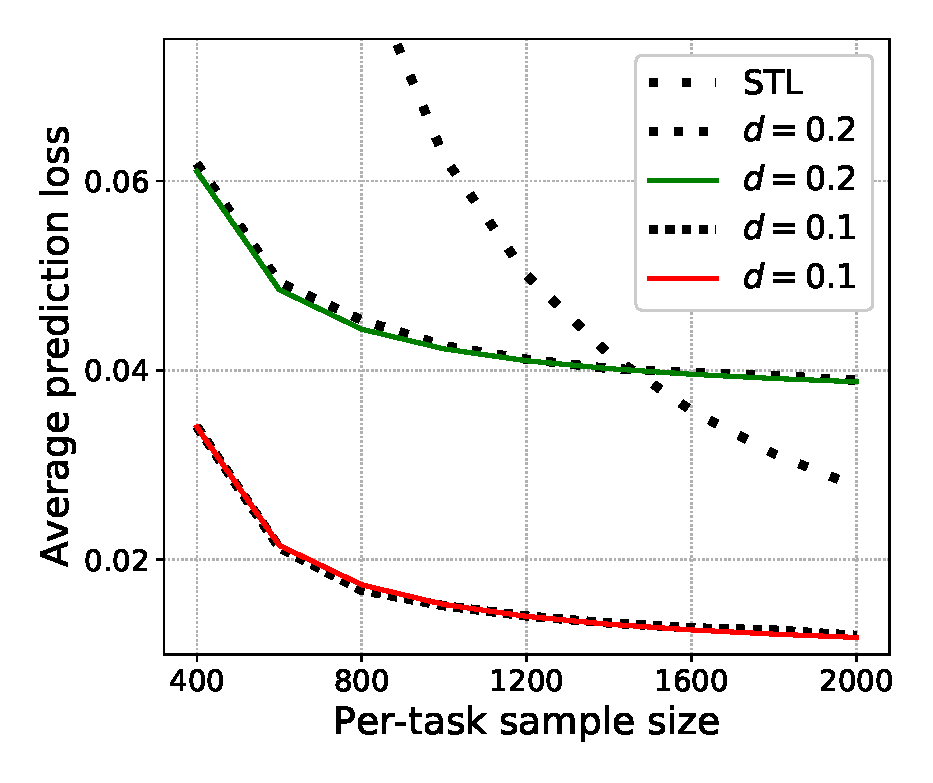
\includegraphics[width=0.9\textwidth]{figures/same_covariates.eps}
		\caption{Example \ref{ex_same_cov}}
		\label{fig_same_cov}
	\end{subfigure}\hfill
	\begin{subfigure}[b]{0.5\textwidth}
		\centering
		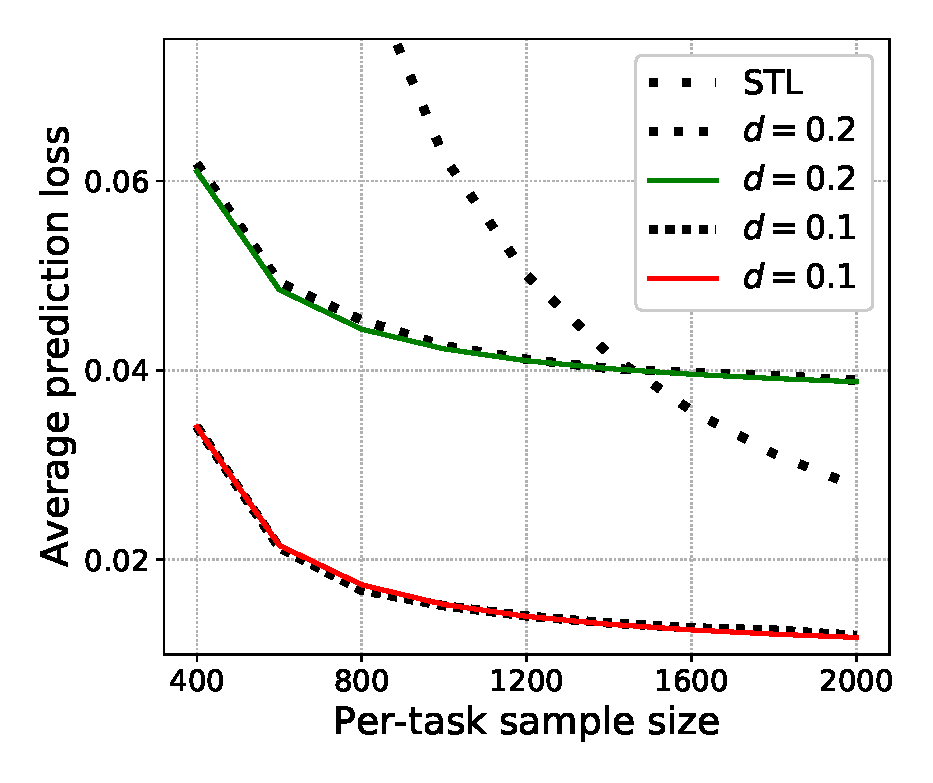
\includegraphics[width=0.9\textwidth]{figures/same_covariates.eps}
		\caption{Example \ref{ex_sample_ratio}}
		\label{fig_width}
	\end{subfigure}
%	\caption{%Three takeaways of our theory in Section \ref{sec_insight}.
%	Our estimated losses (solid line) match the empirical losses (dotted line) accurately under various settings in dimension $p = 200$.
%	\textbf{Left.} Validating Example \ref{ex_same_cov} for ten tasks: the noise variance $\sigma^2$ is $1/4$.
%	\textbf{Middle.} Validating Example \ref{ex_sample_ratio} for two tasks: we discover an interesting phenomena by fixing task two's sample size and increasing task one's sample size.
%	Moreover, our result accurately predicts the critical point (marked in circle) of the loss curve.
%	Depending on how large the distance $d^2$ is, task two's prediction loss decreases initially before increasing again, or decreases monotonically.
%	\textbf{Right.} We show how different levels of covariate shift affect hard parameter sharing when there is no bias.
%	Having covariate shift increases task two's prediction loss when task two's sample size is smaller than task one. Otherwise, having covariate shift (surprisingly) decreases task two's prediction loss.}
%	\label{fig_model_shift_phasetrans}
\end{figure*}

%Moreover, by setting $t=2$ in Theorem \ref{thm_many_tasks}, we can obtain the prediction loss for the HPS estimator for the transfer learning setting where the two tasks have the same covariates  $X^{(1)}=X^{(2)}$. For the reader's convenience, we give the precise statement in Corollary \ref{thm_two_tasks}.
%Theorem \ref{thm_many_tasks} implies Theorem \ref{thm_two_tasks} as a special case with $t=2$ and $r=1$.
%In this section, we consider the setting where the two tasks have the same covariates  $X^{(1)}=X^{(2)}$.
%We define $A^\star \in \R^{2}$ as the normalized eigenvector corresponding to the larger eigenvalue of the $2\times 2$ matrix
%$ {B^\star}^\top \Sigma  B^\star,$ where recall that $B^\star \define [{\beta}^{(1)},{\beta}^{(2)}] \in \real^{p\times 2}$ by definition.
% is the matrix formed by the linear model parameters of the two tasks.
%Without loss of generality, we assume that the two eigenvalues of ${B^\star}^\top \Sigma B^\star$ are not degenerate, so that $A^\star$ is uniquely defined. %Otherwise, Theorem \ref{thm_two_tasks} will give a null result.
%In the following corollary, the estimate \eqref{minimizer_beta1} shows that the minimizer $\hat a$ is approximately equal to $A^\star(1)/A^\star(2)$, while \eqref{Li_multi0} gives the exact asymptotic limit of $L_2(\hat{\beta}_2^{\MTL}(\hat a)) $, together with an explicit convergence rate that we believe to be sharp.

%\begin{corollary}\label{thm_two_tasks}
%Under Assumption \ref{assm_big1}, suppose that $X^{(1)}=X^{(2)}$ and $n_1=n_2\equiv n$. Let $c>0$ be an arbitrary (small) constant. Then we have that with high probability,
%\be\label{minimizer_beta1}
%\left\| u_{\hat a}u_{\hat a}^\top - A^\star {A^\star}^\top\right\|_F  \le  \left[\frac{ n^{-1/2+2/\varphi+c}  \|{B^{\star}}^{\top}\Sigma B^{\star}\|  + n^{-1/2+c} \sigma^2 }{\lambda_1 - \lambda_{2} } \right]^{1/2},
%\ee
%where $u_{\hat a}$ is the unit vector defined as
%$ u_{\hat a}:= \frac1{\hat a^2 +1} \begin{pmatrix} {\hat a}\\ %1\end{pmatrix},$ and $\lambda_1 $ and $\lambda_{2}$ are respectively the larger and smaller eigenvalues of ${B^\star}^\top\Sigma B^\star$.
%for task 2,  % over the randomness of the input,
%Moreover, the prediction loss of the HPS estimator satisfies that with high probability,
%	\begin{align}
%		& \bigabs{L_2(\hat{\beta}_2^{\MTL}(\hat a)) - \left\|(\Sigma^{(2)})^{1/2} \left(A^\star(2) \cdot B^{\star}A^{\star}  - \beta^{(2)}\right)\right\|^2  - |A^\star(2)|^2  \frac{p\sigma^2}{n-p} } \nonumber\\
%		& \le  \left[  \frac{  n^{-1/2+2/\varphi+c} \|{B^{\star}}^{\top}\Sigma B^{\star}\|+n^{-1/2+c} \sigma^2} {\lambda_1  - \lambda_2 }\right]^{1/2}   \left(\norm{\Sigma^{1/2} B^{\star}}^2+  \sigma^2\right), \label{Li_multi0}
		%\le n^{-\frac{c_{\varphi}}2} \cdot \frac{\bigbrace{ \norm{\Sigma^{1/2} B^{\star}}^2+  \sigma^2} \cdot (\bignormFro{\Sigma^{1/2} B^{\star}}^2 + \sigma^2 t)} {\lambda_r ({B^\star}^\top \Sigma B^\star)- \lambda_{r+1}({B^\star}^\top \Sigma B^\star)},
%	\end{align}
%	 where $A^\star(2)$ denotes the second entry of $A^\star$.
%	 \end{corollary}

\begin{example}[How to set the width $r$ in HPS?]
\label{ex_same_cov}
%Suppose every $\beta^{(i)}$ consists of two random components, one that is shared among all tasks and one that is task-specific.
%Thus, each task contributes a certain amount to the shared component and injects a task-specific bias.
%More precisely, %we have
An important question in applications of HPS is how to set the width $r$ of the feature layer.
We use our estimates to show that the optimal width depends on the tradeoff between the estimator's bias and variance.
Concretely, consider a random-effect model where all tasks share a model vector $\beta_0$ plus perturbations.
For every $i=1,2,\cdots, t,$, $\beta^{(i)} = \beta_0 + \wt \beta^{(i)}$, where $\wt \beta^{(i)}$ denotes the $i$-th task-specific component whose entries are i.i.d. Gaussian random variables of mean zero and variance $\frac {\kappa^2} p$.

\begin{claim}
\begin{enumerate}
	\item {\bf Positive vs. negative transfer.} The averaged HPS prediction loss is smaller than the single-task OLS prediction loss if and only if $\frac{d^2}{p}\tr \Sigma  < \frac{p\sigma^2 }{n - p}$, that is, the ``task-specific variance'' is smaller than the ``noise variance'' up to some constant factor.
	
	\item {\bf The optimal rank $r$.} If $\frac{d^2}{p}\tr \Sigma  < \frac{\sigma^2 p}{n - p}$, then the smallest averaged HPS  prediction loss is achieved when $r=1$. Hence increasing the width $r$ of the shared feature representation layer does not help.
\end{enumerate}
\end{claim}
%For our discussion below, we assume that $\kappa^2 \sim d^2 \sim \sigma^2$ and $n\sim p$. %and $d^2=\OO(\kappa^2)$.
%The more precise conditions on the relations between $d^2$, $\sigma^2$ and $\kappa^2$ are given in  \eqref{choiceofpara}.
%We assume that all the random variables have finite moments up to any order as in equation \eqref{assmAhigh2}.
\begin{proof}
    In this random-effect model, using the concentration of Gaussian random vectors (e.g. Lemma \ref{largedeviation} in the supplement  \cite{MTL_suppl}),
    %Based on the definition of the random-effect model,
    the $(i, j)$-th entry of ${B^{\star}}^{\top} \Sigma B^{\star}$ is equal to %(ignoring lower order terms)
    %\begin{align*}
    %	\beta_i^{\top} \beta_j \approx \norm{\beta_0}^2 + \frac{d^2}{2}\delta_{ij},\quad 1\le i,j \le t,
    %\end{align*}
    \begin{align}\label{betaSbeta}
    	\beta_i^{\top}\Sigma  \beta_j =\beta_0^\top \Sigma \beta_0 + \delta_{ij} \frac{d^2 }{p}\tr \Sigma + \OO\left(p^{-1/2+c}\|\beta_0\|^2+ p^{-1/2+c} d^2\right),
    \end{align}
     with high probability for any constant $c>0$. We omit the details to show the error bound using Lemma \ref{largedeviation}.
    %Note that $\norm{\beta_0}^2$ is approximately $\kappa^2$.
    With \eqref{betaSbeta}, it is easy to calculate that with high probability, the eigenvalues of ${B^{\star}}^{\top} \Sigma B^{\star}$ are given by
    $$\lambda_1=\left[1+\OO(p^{-1/2+c})\right]\cdot\left(t \beta_0^\top \Sigma \beta_0  + \frac{d^2}{ p}\tr \Sigma\right) ,$$
    and
    $$ \lambda_i=\left[1+\OO(p^{-1/2+c})\right]\cdot \frac{d^2}{ p}\tr \Sigma , \ \ i=2,\cdots, t.$$ %Therefore, by taking a rank-$1$ approximation of ${B^{\star}}^{\top} B^{\star}$, we get the average prediction loss of $B^{\star} a_i^{\star}$.
    Thus for the best rank-$r$ approximation $A^\star {A^\star}^\top$  of ${B^{\star}}^{\top}\Sigma  B^{\star}$, we have
    $$\bignorm{\Sigma^{1/2} B^{\star} (A^\star {A^\star}^{\top} - \id_{t\times t})}_F^2= [1+\OO(p^{-1/2+c})]\cdot(t-r)\frac{d^2}{ p}\tr \Sigma $$
    with high probability.
    %To see this, recall that $r$ is one and $A^{\star} {A^{\star}}^{\top}$ is the best rank-$1$ approximation of ${B^{\star}}^{\top}\Sigma B^{\star} = {B^{\star}}^{\top} B^{\star}$.
    %Hence, the above expression is equal to the sum of ${B^{\star}}^{\top} {B^{\star}}$'s bottom $t-1$ singular values.
    %In the random-effect model described above, we further assume that $\Sigma$ is isotropic as an example.
    %We show that when the rank $r$ is one, the average prediction loss of hard parameter sharing is as follows
    Then using \eqref{Li_multi2}, we obtain that
    \[ \frac{1}{t}\sum_{i=1}^t L_i(\hat{\beta}_i^{\MTL}) = \bigbrace{1 - \frac{r}{t}} \frac{d^2}{p}\tr \Sigma + \frac{r}{t} \cdot \frac{p\sigma^2 }{n - p} +\oo(\|\beta_0\|^2+d^2 + \sigma^2) ,\quad \text{w.h.p. }\]
    %We describe a proof sketch.
    %First, we show that the bias equation $L(B^{\star} a_i^{\star})$ simplifies to the following
    %\[ \frac{1}{t} \sum_{i=1}^t L(B^{\star} a_i^{\star}) = \frac{1}{t}\normFro{B^{\star} A^{\star} {A^{\star}}^{\top} - B^{\star}}^2 \approx \left(1 - \frac{1}{t}\right) {d^2}{}  . \]
    %Second, using Fact \ref{fact_tr}, one can see that the average variance is
    %\begin{align*}
    %	\frac{1}{t} \sum_{i=1}^t \sigma^2\norm{a_i^{\star}}^2 \bigtr{\Sigma (X^{\top} X)^{-1}} = \frac{\sigma^2}{t} \sum_{i=1}^t \norm{a_i^{\star}}^2 \frac{p}{n - p}
    %	= \frac{1}{t}\frac{\sigma^2 p}{n - p},
    %\end{align*}
    %because $A^{\star}$ has rank-$1$ and $\sum_{i=1}^t \norm{a_i^{\star}}^2 = 1$.
    %Combined together, we have derived the average prediction loss in the random-effect model.
    %If the error is sufficiently small, then
    %Recall that the average prediction loss of STL scales as $\sigma^2\cdot \bigtr{\Sigma (X^{\top} X)^{-1}} = \frac{\sigma^2 p}{n - p}$ by Fact \ref{fact_tr}.
    %Comparing HPS to STL, we have the following qualitative properties.
    %	Suppose $n$ is sufficiently large so that the error is negligible.
\end{proof}
\end{example}



%We demonstrate the accuracy of our results in simulations.
%While our theory is asymptotic (with error terms that are negligible when $p$ is sufficiently large), we observe that they are incredibly accurate in a moderate dimension of $p = 200$.



First, we validate the result of Example \ref{ex_same_cov}.
Figure \ref{fig_same_cov} shows the average prediction loss over ten tasks as we increase the number of samples per-task from $400$ to $2000$.
In all the parameter settings, our results estimate the empirical losses accurately.
We also observe a trend that the average prediction loss increases as we increase distance $d$ from $0.1$ to $0.2$.
Our work explains the differences between these two settings since $d^2 = 0.1^2$ is always smaller than $\frac{\sigma^2 p}{n - p}$, but $d^2 = 0.2^2$ is not.
%Second, when $d = 0.1$, we have that $d^2 \le \frac{\sigma^2 p}{n - p}$ for all values of $n$, hence the average prediction loss of hard parameter sharing is always lower than STL.
Indeed, we observe a crossover point between hard parameter sharing and STL.
Finally, for $d = 0.2$, looking horizontally, we find that HPS requires fewer samples per-task than STL to achieve the same loss level. %\FY{I do not quite understand this sentence about "3x fewer", because how much data needed depends on $d$ and the prediction loss level we are looking at. For example, at the cross point, this ratio is 1. }


%Our result from Corollary \ref{cor_MTL_loss} explains this trend.


%Covariate shift: We set $\kappa = 1$ and $d = 0$.
%We set $\rho_2 = 4$ and vary $\rho_1$ from $5$ to $25$ for sample sizes.
%We use the scale parameter $\lambda = 1$ for the curve without covariate shift and $\lambda = 2$ for the curve with covariate shift (cf. Section \ref{sec_covshift}).


%Recall that Section \ref{sec_data_size} shows that increasing the data size of the source task does not always improve the performance of MTL for the target task.
%In Figure \ref{fig_ab_data}, we show that for source task MR and target task SST, there is a transition from positive to negative transfer as we increase the data size of the source task.
%Our result provides a fine-grained insight on the covariance alignment algorithm proposed in \cite{WZR20}.
%Recall that the covariance alignment procedure in \cite{WZR20} adds an additional module between the word embedding representation and the shared module.
%When the source task data size is particularly large compared to the target task, we show that applying the covariance alignment algorithm results in more significant gains.
%In Figure \ref{fig_ab_cov}, we observe that the benefit from aligning task covariances becomes more significant for LSTM and MLP as we increase the number of datapoints of the source task.

%\begin{table}
%	\begin{center}
%		\begin{tabular}{c c c c c}
%			\toprule
%			\multirow{2}{*}{{\bf Models}} & \multicolumn{2}{c}{\begin{minipage}{1.1in}\begin{center}
%				                                                                          MR, SST, SUBJ, CR, MPQA, TREC\end{center}\end{minipage}} & \multicolumn{2}{c}{\begin{minipage}{1.1in}\begin{center}MR, SST, SUBJ, CR, MPQA\end{center}\end{minipage}} \\
%			\cmidrule(lr){2-3} \cmidrule(lr){4-5}
%			& {\bf Stanford} & {\bf Alignment} & {\bf Stanford} & {\bf Alignment} \\
%			\midrule
%			{\bf MLP}  & > 100\% & 39\% & 25\% & 25\% \\
%			{\bf LSTM} & 36\% & 36\% & 28\% & 25\% \\
			% {\bf CNN}  & 76\% & - & 32\% & -\\
%			\bottomrule
%		\end{tabular}
%	\end{center}
%	\caption{Taskonomy experiment.}
%	\label{tab:taskonomy}
%\end{table}
%\begin{figure}[!t]
%	\centering
%	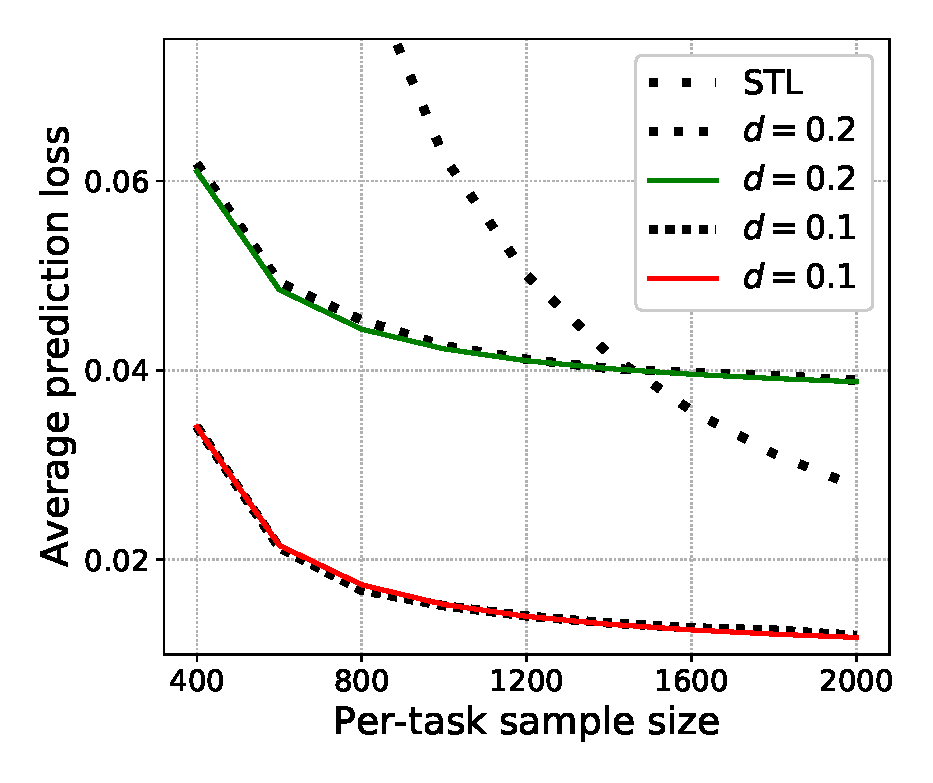
\includegraphics[width=0.35\textwidth]{figures/same_covariates.eps}
%	\caption{Validating Example \ref{ex_same_cov} in Section \ref{sec_same} for $10$ tasks: our estimated loss (solid line) matches the empirical loss (dotted line) accurately for various task-specific variance $d^2$ and sample size $n$ settings. The feature dimension $p$ is $200$, and noise variance $\sigma^2$ is $1/4$.}
%	\label{fig_same_cov}
%\end{figure}





%The estimate \eqref{minimizer_beta1} shows that the minimizer $\hat a$ is approximately equal to $A^\star(1)/A^\star(2)$, while \eqref{Li_multi0} gives the exact asymptotic limit of $L_2(\hat{\beta}_2^{\MTL}(\hat a)) $, together with an explicit convergence rate that we believe to be sharp.


%It is not hard to extend the above result to the cases with more than two tasks. We make this extension for the following reasons. First, it provides a clearer geometric intuition than the two-task setting as we will discuss below. Second, the corresponding multi-task setting is prevalent in applications of multi-task learning to image classification, where there are multiple prediction labels/tasks for every image \cite{chexnet17,EA20}. Finally, it provides useful insights into a more general theory of multi-task learning, which we will explore in greater details in future works.

%We consider an arbitrary local minimum $B, W_1, \dots, W_2$ of the optimization objective.
%We extend the bias-variance decomposition from the two-task case to the multiple-task case.
%We observe that the expected prediction loss of $\hat{\beta}_t^{\MTL}$ conditional on $X$ consists of a bias and a variance equation as follows
%\begin{align}
%	\exarg{\varepsilon_1, \dots, \varepsilon_t}{L(\hat{\beta}_t^{\MTL}) \mid X}
%	=& \bignorm{\Sigma^{1/2} \bigbrace{B^{\star} \cW^{\top} (\cW \cW^{\top})^{-1} W_t - \beta_t}}^2 \label{eq_bias_multiple} \\
%	&+ \sigma^2 \cdot (W_t^{\top} (\cW \cW^{\top})^{-1} W_t) \cdot \bigtr{\Sigma (X^{\top} X)^{-1}} \label{eq_var_multiple}
%\end{align}
%One can see that equation \eqref{eq_bias_multiple} is the bias of the multi-task learning estimator and equation \eqref{eq_var_multiple} is its variance.
%Compared to the prediction loss of single-task learning (cf. equation \eqref{eq_var_stl}), we observe that the variance equation \eqref{eq_var_multiple} is always smaller because $W_t^{\top} (\cW \cW^{\top})^{-1} W_t \le 1$.
%On the other hand, the bias equation \eqref{eq_bias_multiple} is always larger because of the difference between the task models.
%We show the generalization error of hard parameter sharing estimators.
%Before stating the result, we define the following notations.




%The key step for proving Theorem \ref{thm_many_tasks} is a characterization of $f(A, B)$'s global minimizer.
%\medskip
%
%\noindent\textbf{Comparison to single-task learning (STL).}
%Theorem \ref{thm_many_tasks} provides a sharp generalization error bound that is asymptotically tight when $n$ goes to infinity.
%%The limiting loss of hard parameter sharing consists of two parts, a bias term $L(B^{\star} a_i^{\star})$ that measures the error of $B^{\star} a_i^{\star}$, and a variance term that scales with noise variance $\sigma^2$.
%%	Our result implies that the variance of hard parameter sharing is always smaller than single-task learning.
%%	This is because	STL's variance is equal to $\frac{\sigma^2 \cdot p} {n - p}$ by Fact \ref{lem_minv}, and $\norm{a_i^{\star}}^2 \le 1$ since the spectral norm of $U_r$, which is a projection matrix, is at most one.
%One direct implication of our result is that compared to STL, the variance always decreases, since STL's variance is equal to $\sigma^2 \tr[\Sigma (X^{\top} X)^{-1}]$.
%On the other hand, the bias always increases.


%\FY{add simulations to check our results; discuss motivations and possible applications}
\iffalse
In this paper, we consider a natural extension of the estimator $\hat \beta^{\rm{TL}} $, that is, the \emph{hard parameter sharing} (HPS) estimator, which has been a standard type of estimator in multi-task learning \FY{citations}. More precisely, we study the following HPS architecture: a shared feature representation layer $B\in\real^{p}$ for all datasets and a separate output layer $A_i \in \real$ for every dataset $i$. Then we study the following minimization problem:
\begin{align}\label{eq_tsl}
			f(A, B) = \norm{X^{(1)} B A_1 - Y^{(1)}}^2 + \norm{X^{(2)} B A_2 - Y^{(2)}}^2,
\end{align}
where we abbreviate $A = [A_1, A_2]$. Let $(\hat{A}, \hat{B})$ be the minimizer of $f(A, B)$. We define the hard parameter sharing (HPS) estimator for task $i$ as
\be\label{def_HPS}\hat{\beta}_i^{\MTL} = \hat{B} \hat{A}_i,\quad i=1,2.\ee
Note that $\hat \beta^{\rm{TL}}$ is a special case of $\hat{\beta}_i^{\MTL}$ by setting $A_1=A_2=1$.

For the optimization objective $f(A, B)$ in \eqref{eq_tsl}, using the local optimality condition $\frac{\partial f}{\partial B} = 0$, we can solve that
	\begin{align}
		\hat{B} = A_2^{-1} \hat \Sigma(a)^{-1} \left[a (X^{(1))})^{\top}Y^{(1)} +  (X^{(2)})^{\top}Y^{(2)}\right], \label{eq_Bhat_2task} %\\
		%&= (B^\star A ^{\top}) (A A^{\top})^{-1} + (X^{\top}X)^{-1}X^{\top}   \bigbrace{\sum_{j=1}^t \varepsilon_i A_i^{\top}} (A  A^{\top})^{-1}.
	\end{align}
where we denote $a:=A_1/A_2$ and $\hat \Sigma(a):= a^2 (X^{(1)})^\top X^{(1)}  + (X^{(2)})^\top X^{(2)}$.
Applying $\hat B$ to equation \eqref{eq_tsl}, we obtain an objective that only depends on $a $ as follows %\HZ{$A$ has been used to denote the output layers. Could you replace $A$ with another symbol (say $x$)?}
 \begin{align}
		 g(a) \define & \left\| X^{(1)} \hat\Sigma(a)^{-1} (X^{(2)})^\top X^{(2)} (a\beta^{(2)}-\beta^{(1)}) \right. \nonumber\\
			& \left. + \left(a^2 X^{(1)}\hat \Sigma(a)^{-1} (X^{(1)})^\top-\id_{n_1\times n_1}\right)\epsilon^{(1)}+ a X^{(1)}\hat \Sigma(a)^{-1} (X^{(2)})^\top \epsilon^{(2)} \right\|^2 \nonumber\\
		   +& \left\| X^{(2)} \hat \Sigma(a)^{-1} (X^{(1)})^\top X^{(1)} (a\beta^{(1)}-a^2\beta^{(2)}) \right. \nonumber\\
		  &\left.+ \left(X^{(2)}\hat\Sigma(a)^{-1} (X^{(2)})^\top-\id_{n_2\times n_2}\right)\epsilon^{(2)} + a X^{(2)}\hat \Sigma(a)^{-1} (X^{(1)})^\top \epsilon^{(1)} \right\|^2. \label{eq_mtl_A12}
	\end{align}
Let $\hat a$ be the minimizer of $g(a)$. Throughout this paper, we regard $Y^{(1)}$ as the source data, and $Y^{(2)}$ as the target data.  Then the HPS estimator \eqref{def_HPS} for the target task 2 is
\be\label{HPS_est}
\hat{\beta}_2^{\MTL} (\hat a) = \hat \Sigma(\hat a)^{-1}  \left[\hat a (X^{(1))})^{\top}Y^{(1)} +  (X^{(2)})^{\top}Y^{(2)}\right].
\ee
\fi

	\section{Empirical results}


%\subsection{Comparison between the averaging and HPS estimators}
\paragraph{Regression tasks.}

\paragraph{Text classification.}
Our results and simulations are all in the high-dimensional linear regression setting.
How well do they extend to other scenarios?
In this section, we conduct further studies on six text classification datasets.
Our datasets include a movie review sentiment dataset (MR) \cite{pang2005seeing}, a sentence subjectivity dataset (SUBJ) \cite{pang2004sentimental}, a customer reviews dataset (CR) \cite{hu2004mining}, a question type dataset (TREC) \cite{li2002learning}, an opinion polarity dataset (MPQA) \cite{wiebe2005annotating}, and the Stanford sentiment treebank (SST) dataset \cite{socher2013recursive}.
%The question is to predict positive or negative sentiment expressed in the text.
Our model consists of a word embedding layer with GloVe embeddings \cite{pennington2014glove} followed by a long-short term memory (LSTM) or a multi-layer perception (MLP) layer \cite{lei2018simple}.\footnote{For MLP, we apply an average pooling layer over word embeddings. For LSTM, we add a shared feature representation layer on top of word embeddings.}


\subsection{Covariate alignment}


\paragraph{Covariate shift}
Recall from Example \ref{ex_covshift} that having covariate shifts worsens the variance (hence the loss) of hard parameter sharing when the sample ratio increases.
This highlights the need for correcting covariate shifts when the sample size ratio rises.
To this end, we study a covariance alignment procedure proposed in \cite{WZR20}, designed to correct covariate shifts.
The idea is to add an alignment module between the input and the shared module $B$.
This module is then trained together with $B$ and the output layers. We refer to \cite{WZR20} for more details about the procedure and the implementation.
%We validate our insight on this procedure in the experiments.
%We implement the covariance alignment procedure following \cite{WZR20}.

We conduct multi-task training on all $15$ task pairs from the six datasets.
In Figure \ref{fig_ab_cov}, we measure the performance gains from performing covariance alignment vs. HPS.
To get a robust comparison, we average the improvements over the 15 task pairs.
The result shows that as the sample size ratio increases, performing covariance alignment provides more significant gains over HPS.
We fix task two's sample size at $1,000$, and increase task one's sample size from $1,000$ to $3,000$.



%One estimator that is sometimes employed in the literature is simply an average of the OLS estimators for two tasks \cite{bastani2020predicting}
%\be\label{eq_est_ave}\hat \beta^{\AV}(\lambda)=\lambda \cdot \hat \beta_1^{\STL}+ (1-\lambda)\cdot \hat \beta_2^{\STL},\ee
%where $\lambda\in [0,1]$ is an averaging parameter subject to choice in practice, and we recall that the OLS estimators are given by
%$$\hat \beta_i^{\STL}= [(X^{(i)})^\top X^{(i)}]^{-1}(X^{(i)})^\top Y^{(i)},\quad i=1,2.$$
%The estimator in \eqref{eq_est_ave} is conventionally called an \emph{averaging estimator}.
%In particular, when $\lambda=0$ and $1$, we get the OLS estimators for tasks 2 and 1, respectively.

%\section{Experimental results}

\subsection{Progressive training}%\label{sec_text}


%multi-layer perceptron (MLP), LSTM, CNN on all tasks
%We use this task to verify our theoretical results on model capacity and task covariance in real world.
%{\it ChestX-ray14.} This dataset contains 112,120 frontal-view X-ray images \cite{chexnet17}.
%There are 14 diseases (tasks) for every image that we would like to predict.
%We use densenet121 as the shared module \cite{huang2017densely}.
%We treat each label as one task a binary classification problem and formulate it as a 14-task multi-task learning problem.
%This dataset is curated where the labels
%We use the CheXNet model from~\cite{chexnet}, which is a 121-layer convolutional neural network on all tasks.
%For the text classification experiment, we encode each word using the GLoVe word embeddings.%
%\footnote{http://nlp.stanford.edu/data/wordvecs/glove.6B.zip}
%We evaluate three model choices.
%\textit{Predicting transfer effect via STL results.}
%We show that the single-task based metric proposed in Section \ref{sec_similarity} can predict positive or negative transfer in MTL.
%A common challenge in the study of MTL is that the results can be hard to understand.
%It is difficult to predict when MTL performs well without running extensive trials.
%Our insight is that we can use STL results to help understand MTL results.
%Table \ref{tab:mtl_better_than_stl} shows the result on both the sentiment analysis and the ChestX-ray14 tasks.
%We find that using a threshold of $\tau = 0.1$, the STL results correctly predict positive or negative transfer with $75.6\%$ precision and $38.8\%$ recall among $30$ times $5$ (random seeds) task pairs!
%We observe similar results for $91$ task pairs from the ChestX-ray14 dataset.
%The results show that STL results are indicative of MTL results.

\paragraph{Sample size ratio.}
First, we we show that our observation in Figure \ref{fig_size} also occurs in the text classification tasks.
In Figure \ref{fig_ab_data}, we observe that for multiple example task pairs, increasing task one's sample size improves task two's prediction accuracy initially, but hurts eventually.
On the $y$-axis, we plot task two's test accuracy using HPS, subtracted by its STL test accuracy.
%validate that as we increase the sample ratio while keeping task two's sample size fixed, task two's prediction accuracy does not always increase.
We fix task two's sample size at $1000$ and increase task one's sample size from $100$ to $3000$.

These examples and the one in Figure \ref{fig_size} suggest a natural progressive training schedule, where we add samples progressively until performance drops.
Concretely, here is one implementation of this idea.
%In particular, Figure \ref{fig_size} (and our analysis) shows that $L(\hat{\beta}_t^{\MTL})$ behaves as a quadratic function over $\rho_1$.
%More generally, depending on how large $\Psi(\beta_1, \beta_2)$ is, $L(\hat{\beta}_t^{\MTL})$ may also be monotonically increasing or decreasing.
%Based on this observation, we propose a progressive training schedule to improve the compuational efficiency of hard parameter sharing.
\begin{itemize}
	\item We divide the training data into $S$ batches.
	We divide the training procedure into $S$ stages. During every stage, we progressively add one more data batch.
	\item During every stage, we train for $T$ epochs using only the $S$ batches. If the validation accuracy drops compared to the previous round's result or reach a desired threshold $\tau$, we terminate.
%	Algorithm \ref{alg_inc_train} in Appendix \ref{app_experiments} describes the procedure in detail.
\end{itemize}
If we apply this procedure to the settings of Figure \ref{fig_ab_data} and \ref{fig_size}, it will terminate once reaching the optimal sample ratio.
%See Algorithm \ref{alg_inc_train} for a complete description for two tasks.
The advantage of this procedure is that it reduces the computational cost compared to standard round-robin training schedules.
For example, if the procedure terminates at 30\% of all batches, then SGD only passes over 30\% of its data, whereas standard round-robin training passes over 100\% of task one's data.

\begin{algorithm}[!t]
	\caption{An incremental training schedule for efficient multi-task learning with two tasks}
	\label{alg_inc_train}
	\begin{algorithmic}[1]
		\Input Two tasks $(X_1, Y_1)$ and $(X_2, Y_2)$.
		\Param A shared module $B$, output layers $W_1, W_2$ as in the hard parameter sharing architecture.
		\Req \# batches $S$, epochs $T$, task $2$'s validation accuracy $\hat{g}(B; W_2)$, a threshold $\tau\in(0,1)$.
		\Output The trained modules $B, W_2$ optimized for task $2$.
		\State Divide $(X_1, Y_1)$ randomly into $S$ batches: $(x^{(1)}, y^{(1)}), \dots, (x^{(S)}, y^{(S)})$.
		\For{$i = 1,\dots, S$}
		\For{$j = 1,\dots, T$}
		\State Update $B, W_1, W_2$ using the training data $\set{x^{(k)}, x^{(k)}}_{k=1}^i$ and  $(X_2, Y_2)$.
		\EndFor
		\State Let $a_i = \hat{g}(B; W_2)$ be the validation accuracy.
		\If{$a_i < a_{i-1}$ or $a_i > \tau$}
		\State \textbf{break}
		\EndIf
		\EndFor
	\end{algorithmic}
\end{algorithm}

%We fill in the details of the experimental procedure used for the results in Figure \ref{fig_ablation}.
%\squishlist
%	\item Task similarity: We select a similar and a dissimilar source task compared to the target task using domain knowledge.
%First pair: the customer review dataset (CR) , which predicts whether a review is positive or negative, is more similar to SST (sentiment treebank) than MPQA (question type).
%Second pair: SST is more similar to MR since they both concern about positive or negative opinions expressed the text.
%TREC is less similar to MR because the task is about question types.
%Third pair: MPQA (opinion polarity) is more similar to TREC (question type)
We evaluate the progressive training procedure on the six text classification datasets.
First, we conduct multi-task training over all $15$ two-task pairs from the six datasets.
We focus on task two's test accuracy and set $\tau$ as task two's test accuracy obtained via the standard round-robin training schedule.
We include all of task two's data and progressively add task one's data using the procedure described above.
Since the prediction accuracy has been controlled the same, we compare the computational cost.
We find that when averaged over all $15$ two-task pairs, this procedure requires only $45\%$ of the computational cost to reach the desired accuracy $\tau$ for task two.
%Our insight is that since adding more samples from the source task does not always help, we can improve efficiency by adding source samples \textit{progressively} during training.
%\textbf{Improving transfer learning training efficiency.}
%We show that Algorithm \ref{alg_inc_train} also applies to transfer learning settings.
%Compared to fine-tuning the source model on the target task, we show that our proposed method reduces the computional cost by \alert{$xx\%$}, without sacrificing accuracy.
Second, we conduct multi-task training on all six datasets jointly.
We extend our procedure to all six datasets. We include the data from all tasks except SST. For SST, we progressively add data similar to the above procedure.
We set $\tau$ to be the average test accuracy of all six tasks obtained using standard round-robin training.
We find that adding samples progressively from SST requires less than $35\%$ of the computational cost to reach the same average test accuracy $\tau$.

\subsection{Width selection}
%As a further validation, excluding TREC, we observe similar comparative results.
%The data efficiency ratio of using MLP is $100\%$ because the average performance of MTL is worse than the average of STL.
%We further show that applying incremental training helps reduce the data efficiency ratio to \alert{$xx\%$}.
%If TREC is not included, we see that only $25\%$ of the labeled data is needed.



%	\begin{subfigure}[b]{0.33\textwidth}
%		\centering
%		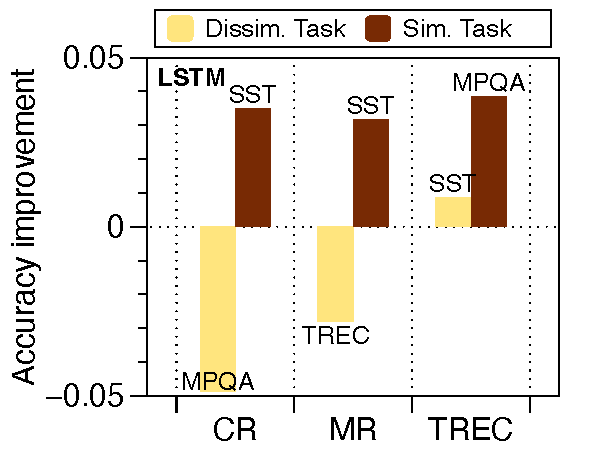
\includegraphics[width=0.975\textwidth]{figures/task_sim_norm_lstm.pdf}
%		\caption{Task similarity}
%		\label{fig_ab_sim}
%	\end{subfigure}%
%	\caption{Validating the three results of Section \ref{sec_insight} on sentiment analysis tasks. (a) Adding a semantically similar source task in MTL performs better than adding a dissimilar task.
%	(b) As source/target sample ratio increases, we observe a transition from positive to negative transfer.
%	(c)
%	Note: (S) denotes the source task and (T) denotes the target task.}


%\begin{minipage}[t]{.58\textwidth}
%	\vspace{-0.1in}
%	\centering
%  \begin{tabular}{c c c c c}
%	\toprule
%		\multirow{2}{*}{{\bf Threshold}}  & \multicolumn{2}{c}{{\bf Sentiment
%		analysis}} & \multicolumn{2}{c}{{\bf ChestX-ray14}} \\
%		& Precision &  Recall & Precision &  Recall \\
%		\cmidrule(lr){1-1} \cmidrule(lr){2-3} \cmidrule(lr){4-5}
%		0.0 & 0.596 & 1.000 & 0.593 & 1.000 \\
%		0.1 & \textbf{0.756} & \textbf{0.388} & \textbf{0.738} & \textbf{0.462} \\
%		0.2 & 0.919 & 0.065 & 0.875 & 0.044 \\
		% 0.3 & 1.000 & 0.004 &     - &     - \\
%	\bottomrule
%	\end{tabular}
%	\vspace{0.1in}
%	\captionof{table}{Single-task learning results can help predict postive or negative transfer in multi-task learning.}
%	\label{tab:mtl_better_than_stl}
%\end{minipage}%
%\quad



%\begin{figure}[!t]
%	\centering
%	\begin{subfigure}[b]{0.5\textwidth}
%		\centering
%		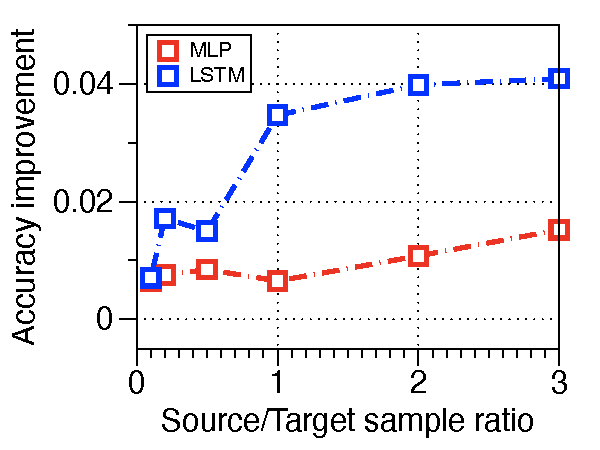
\includegraphics[width=0.5\textwidth]{figures/ratio_alignment_norm_diff_all.pdf}
%		\caption{Averaged over all 16 task pairs}
%		\label{fig_ab_cov}
%	\end{subfigure}\hfill
%	\begin{subfigure}[b]{0.5\textwidth}
%		\centering
%		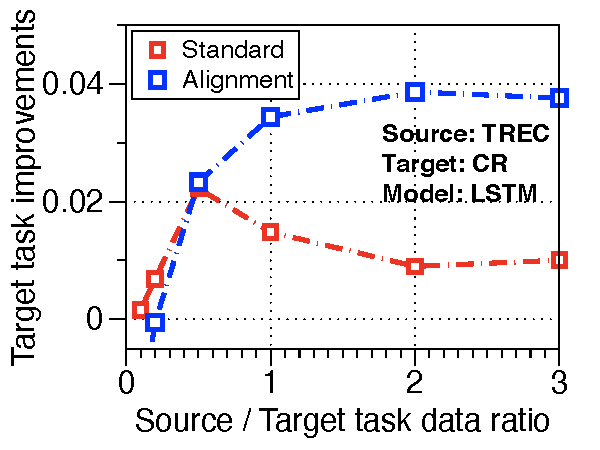
\includegraphics[width=0.5\textwidth]{figures/ratio_alignment_norm_trec_cr_lstm.pdf}
%		\caption{An example task pair}
%		\label{fig_cov_a}
%	\end{subfigure}
%	\caption{ (TREC and CR)}
%\end{figure}

%\textbf{Further results of the covariance alignment procedure.}
%Our results in Figure \ref{fig_ab_cov} are averaged over all the task pairs.
%In Figure \ref{fig_covariate_app}, we show two task pairs as examples.
%In Figure \ref{fig_cov_a}, we observe that for the particular task pair, covariance alignment provides more significant gains when the sample ratio is large.
%In Figure \ref{fig_cov_b}, we observe that covariance alignment does not always improve over the baseline multi-task learning model.
%One explanation is that MR and SST are similar tasks, hence adding the alignment module is unnecessary.
%An interesting question is to understand when adding the alignment module benefits the multi-task learning model.
%We leave this question for future work.
%Note: For text classification tasks, the source task training data size ranges from 500 to 1,500 and target task training data size is 1000; For ChestX-ray14,

%\begin{figure}[!h]
%	\centering
%	\begin{subfigure}[b]{0.48\textwidth}
%		\centering
%		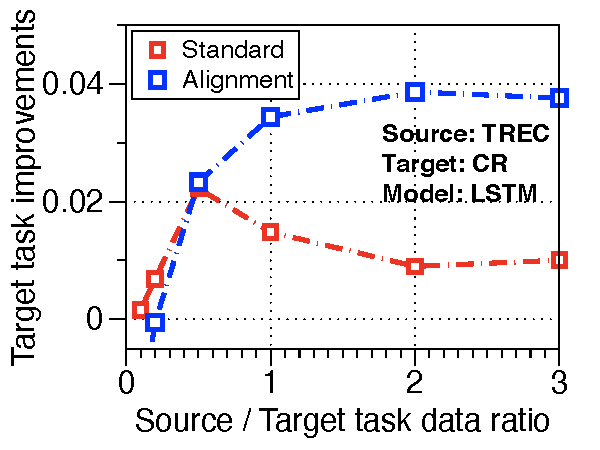
\includegraphics[width=0.7\textwidth]{figures/ratio_alignment_norm_trec_cr_lstm.pdf}
%		\caption{Task pair TREC and CR}
%		\label{fig_cov_a}
%	\end{subfigure}\hfill
%		\begin{subfigure}[b]{0.48\textwidth}
%		\centering
%		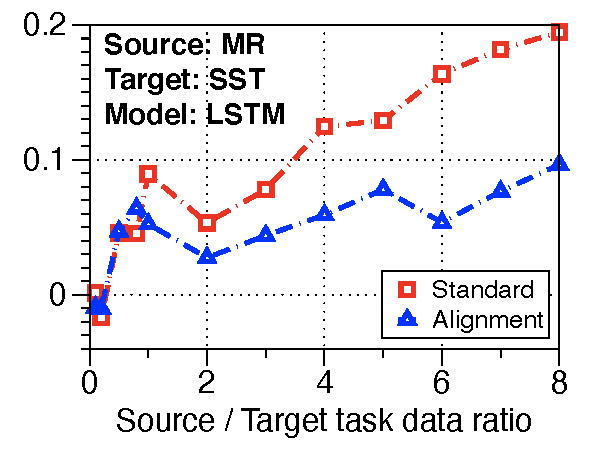
\includegraphics[width=0.7\textwidth]{figures/ratio_alignment_mr_sst_lstm.pdf}
%		\caption{Task pair MR and SST}
%			\label{fig_cov_b}
%	\end{subfigure}
%	\caption{(a) For the task pair TREC and CR, adding the covariance alignment procedure provides more improvement when the source/target sample ratio is large.
%	(b) For the task pair MR and SST, adding the covariance alignment procedure hurts performance.
%	One explanation is that MR and SST are similar tasks, hence adding the alignment module is unnecessary.}
%	\label{fig_covariate_app}
%\end{figure}


\begin{figure}%[!t]
	\begin{subfigure}[t]{0.5\textwidth}
		\centering
		\vspace{0pt}
		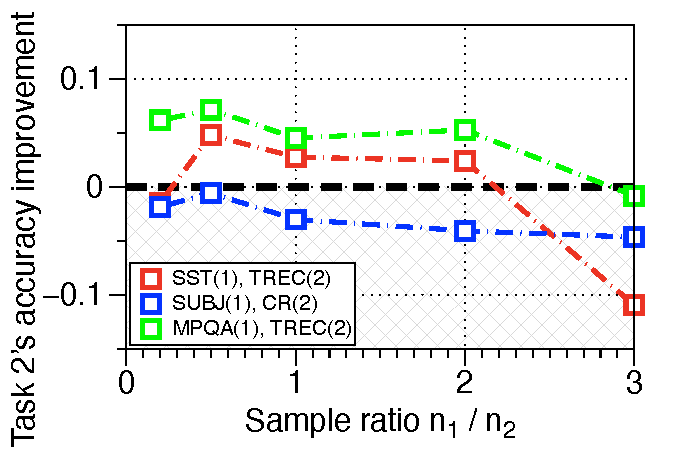
\includegraphics[width=0.8\textwidth]{figures/fig3a.pdf}
		\caption{HPS vs. STL}
		\label{fig_ab_data}
	\end{subfigure}\hfill
	\begin{subfigure}[t]{0.5\textwidth}
		\centering
		\vspace{0pt}
		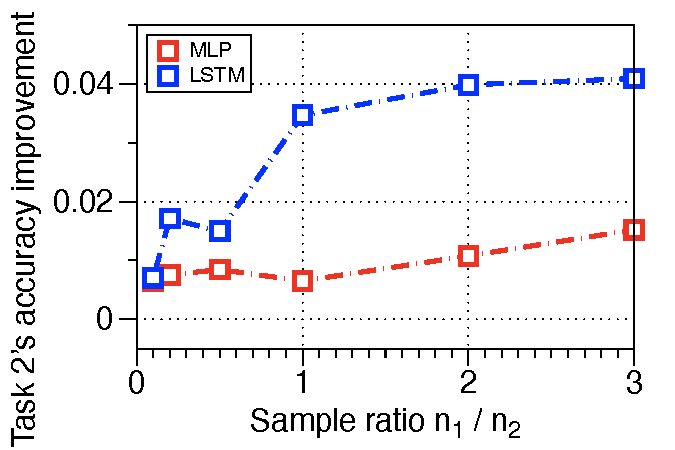
\includegraphics[width=0.8\textwidth]{figures/fig3b.pdf}
		\caption{HPS vs. covariance alignment}
		\label{fig_ab_cov}
	\end{subfigure}
	\caption{Comparing hard parameter sharing (HPS) to single-task learning (STL) and a covariance alignment approach proposed by \cite{WZR20}:
	In Figure \ref{fig_ab_data}, we observe that for multiple task pairs, increasing task one's sample size improves task two's prediction accuracy initially, but hurts eventually -- a phenomenon similar  to Figure \ref{fig_size}.
	In Figure \ref{fig_ab_cov}, we observe that as task one's sample size increases, covariance alignment improves more over HPS.}
	\label{fig_text}
%	\begin{minipage}[t]{0.4\textwidth}
%		\centering
%		\vspace{0pt}
%		\begin{tabular}{c c c}
%		\toprule
		% \multirow{2}{*}{{\bf Models}} & \multicolumn{2}{c}{\begin{minipage}{1.2in}\begin{center}
		% Sentiment\\ analysis\end{center}\end{minipage}} \\
%		\multirow{2}{*}{{\bf Models}} & \multicolumn{2}{c}{\bf Sentiment analysis} \\
		% \cmidrule(lr){2-3}
%		& all tasks & w/o TREC \\
%		\midrule
%		{\bf MLP}  & 31\% & 29\% \\
%		{\bf LSTM} & 35\% & 34\% \\
%		{\bf CNN}  & 30\% & 28\% \\
%		\bottomrule
%		\end{tabular}
%		\captionof{table}{Finding the best sample ratio via a progressive training schedule.}
%		\label{tab:taskonomy}
%	\end{minipage}
\end{figure}

%\begin{algorithm}[!t]
%	\caption{A progressive training schedule given two tasks}
%	\label{alg_inc_train}
%	\begin{algorithmic}[1]
%		\Input Two tasks $(X^{(1)}, Y^{(1)})$ and $(X^{(2)}, Y^{(2)})$.
%		\Param A shared module $B$, output layers $A_1, A_2$ as in the hard parameter sharing architecture.
%		\Req \# batches $S$, epochs $T$, task $2$'s validation accuracy $\hat{g}(B; W_2)$, a threshold $\tau\in(0,1)$.
%		\Output The trained modules $B, A_2$ optimized for task $2$.
%		\State Divide $(X^{(1)}, Y^{(1)})$ randomly into $S$ batches: $(x^{(1)}, y^{(1)}), \dots, (x^{(S)}, y^{(S)})$.
%		\For{$i = 1,\dots, S$}
%			\For{$j = 1,\dots, T$}
%				\State Update $B, A_1, A_2$ using the training data $\set{x^{(k)}, x^{(k)}}_{k=1}^i$ and  $(X^{(2)}, Y^{(2)})$.
%			\EndFor
%			\State Let $a_i = \hat{g}(B; A_2)$ be the validation accuracy.
%			\If{$a_i < a_{i-1}$ or $a_i > \tau$}
%				\State \textbf{break}
%			\EndIf
%		\EndFor
%	\end{algorithmic}
%\end{algorithm}
	\section{Conclusions and Discussions}\label{sec_conclude}

This work studied the generalization properties of a widely used hard parameter sharing approach for multi-task learning.
We provided sharp bias-variance tradeoffs of HPS in high-dimensional linear regression.
Using these results, we analyzed how varying sample sizes and covariate shifts impact HPS.
We rigorously explained several empirical phenomena such as negative transfer and covariate shift related to these dataset properties.
We validated our theory and conducted further studies on text classification tasks.

We describe several open questions for future work.
%First, it would be interesting to tighten our estimate in Corollary \ref{cor_MTL_loss}, which would extend the observation in Figure \ref{fig_size} to small $n_1$.
%Second, it would be interesting to extend our result to classification problems such as logistic regression.
First, our result in Corollary \ref{cor_MTL_loss} involves an error term that scales down with $n_1$.
Tightening this error bound requires showing the limit of $\normFro{({Z^{(1)}}^{\top} Z^{(1)} + {Z^{(2)}}^{\top} Z^{(2)})^{-1} {Z^{(1)}}^{\top} Z^{(1)}}^2$ for two isotropic sample covariance matrices.
This requires studying the asymptotic singular values distribution of the non-symmetric matrix $({Z^{(1)}}^{\top} Z^{(1)})^{-1}{Z^{(2)}}^{\top} Z^{(2)}+\id$, which is still an open problem in random matrix theory.
%FY: $+\id$ is very important and makes the problem very hard; otherwise the problem can be solved with current RMT methods.
The eigenvalue distribution of this matrix, which has been obtained in \citet{Fmatrix}, might help resolve this problem.
%but its singular values will follow a different distribution since the matrix is not symmetric.
 %might require new techniques beyond the current ones in random matrix theory .%\HZ{to add}.
Second, it would be interesting to extend our results to classification problems.
Several recent work has made remarkable progress for logistic regression in the high-dimensional setting (e.g. \citet{sur2019modern}).
It is an interesting question to study logistic regression in a multiple-sample setting.


	\bibliographystyle{plainnat}
	\bibliography{rf,rf_tl,ref_mtl}

\end{document}